\documentclass[paper=a5,listof=totoc]{scrartcl}
\usepackage{xcolor}
\usepackage{hsbcommon}
\usepackage[hidelinks=true]{hyperref}
\usepackage{multicol}

\usepackage[scale=3,colorspec=0.96,text=internal~use~only]{draftwatermark}

\usepackage[headsepline]{scrlayer-scrpage}

\usepackage[utf8]{inputenc}
\usepackage{setspace}
\usepackage{biblatex}
\usepackage{eurosym}
\addbibresource{literature.bib}
\usepackage{pgfplots}
\pgfplotsset{width=7cm,compat=1.18}
\tikzset{->/.style={-Latex}}

%% define the dates
\newcommand{\mysession}[1]{%
  \ifcase#1\relax\or
    April 13th\or
    April 20th\or
    May 4th\or
    May 11th\or
    May 18th\or
    June 1st\or
    June 8th\or
    June 15th\or
    June 22nd\or
    June 26th (Friday)\or
    June 29th\or
    July 6th\or
    \else
  \fi
}

\title{Micro-Economics}
\author{
\includegraphics[width=4cm]{../shared/img/1600px-Logo_HSB_Hochschule_Bremen_cropped.png}\\Jan Suchanek}
\date{Summer Semester \the\year\\\today}

\automark{section}
\pagestyle{scrheadings}
\ihead{\leftmark}
   \chead{}
   \ohead{Microeconomics}

\setlength{\parskip}{1ex}

\begin{document}

\onehalfspacing

\maketitle

\begin{abstract}
    This is the script for the module Microeconomics / Introduction to Economics, as taught at \noun{Hochschule Bremen}, Summer Semester 2026. It is a $1:1$ white-cover version of the slides. A hand \faHandPointRight\ indicates slide changes.

    The module covers the most important aspects of Microeconomics, and it does so in a visual manner, with a minimum of algebra.

    AI has not been used for content creation, but for refactoring \LaTeX\ code and to generate the control questions in the annex.

    This is work in progress.
\end{abstract}

\newpage

\tableofcontents

\clearpage

% \section{Organisation and Module Walkthrough}

\begin{frame}{Introduction}
    \mycomment{I am honoured to teach you this semester.  I have an extensive background in academia and as a consultant and manager.}
    \mytext{
    Jan Suchanek
    \begin{itemize}
        \item Diplom-Volkswirt (MA Economics)
        \item MBL (Master of Business Law)
        \item based in Berlin, born in Hamburg
        \item English, German (native), French, Spanish
        \item work as consultant, project manager, lecturer
        \item Project Manager: Energy Networking Projects
        \item Teaching Project Management
        \item Teaching Foreign Trade (ISGM)
        \item ...and this class
    \end{itemize}
    }
\end{frame}

\begin{frame}{Introduction}
    \mytext{
    Attendants:
        \begin{itemize}
            \item BIM students
            \item Incoming Students?
            \item favourite market?
        \end{itemize}
    }
\end{frame}

\begin{frame}{Schedule, Grading and Procedure}
    \mycomment{This class is predominantly an online class. There are, however, some sessions held in situ.

    Lectures will cover the theory. Student presentations shall provide the illustration from real life applications by outlining the most important properties of specific markets. 
    
    }
    \mytext{
        \begin{itemize}
            \item April -- July: online lectures
            \item Mai 18th,  Room D207
            \item[] Student Present a Market (early bird)
            \item June 26th \& June 27th (Saturday!) Room D107
            \item[] Student Present a Market (last chance)
            \item End July: Written Exam
        \end{itemize}

        % \medskip
        
        \begin{description}
            \item[50\%] Student Presentation 
            \item[50\%] digitally written exam 
        \end{description}
    }
\end{frame}

\begin{frame}{Schedule, Grading and Procedure}
    \mytext{
        \begin{itemize}
            \item Students present a market
            \item groups per 1-5 students
            \item 15 minutes presentation, 5 minutes discussion
            \item Two options:
            \begin{enumerate}
                \item Early bird -- Mai 18th (max. 8 gr.)
                \item Last chance -- June 26th and 27th
            \end{enumerate}
            \item state your intentions on forum (\href{}{LINK})
        \end{itemize}

    }
    
    \mycomment{
        Every student must speak over one slide / cover one aspect. 
        
        Grading will be 50\% overall quality and consistence of the presentation and 50\% individual performance.    
    } 
    
\end{frame}



\begin{frame}{Economic Theory}
    \showmytikz{../shared/tikz/tikz-tree1-micromacro.tex}
    \mycomment{
        \begin{itemize}
            \item Micro-Economics looks at individuals
            \item Micro-Economics looks at single transactions
            \item Micro-Economics looks at single markets
            \item Micro Economics looks at \textit{partial equilibria}, i.e. equilibria of single markets
            \item Micro-Economics are foundational for Economics
            \item Macro-Economics looks at the economy: aggregates
            \item Macro-Economics looks at the \textit{total equilibrium}, e.g. of the economy as a whole.
        \end{itemize}
        }
\end{frame}

\begin{frame}{Microeconomics within Economics}
    \showmytikz{../shared/tikz/tikz-tree2-micromacro.tex}
        \mycomment{
            Micro-economics looks at the fundamentals of economic behaviour under idealised circumstances.

            
            Micro-economics looks at isolated (and idealised) individual effects, not at the economy as an entire system.            
        }
\end{frame}
\begin{frame}{Macroeconomics within Economics}
    \showmytikz{../shared/tikz/tikz-tree3-micromacro.tex}
        \mycomment{
            Macroeconomics looks at the economy as a circular system. There are topics belonging to both branches, and Microeconomics provide the fundamentals for Macroeconomics. However, the sum is more than its parts.         
        }
\end{frame}

\begin{frame}{Economic Theory}
    \mycomment{
        In physics, the falling of objects can be best understood by abstracting from the presence of air resistance to isolate the pure effect of gravity. 
        
        Economics takes a similar approach. Starting from first principles, Microeconomics analyses optimal choices and their welfare results in a generalised manner.
                
        % There is also the empiric branch, and applied Economics.
        
        Among empirical economics is econometrics, statistics, also modelling (of concrete cases), hence forecasting, among with advice and consultancy to public and private entities, and the study of economic history.

        Of course, theory is helpful for empirical studies, and for policy analysis and normative recommendations.
    }
    \mytext{
        \begin{center}
            Micro-Economics is in Economics 
            
            \textit{almost like}
            
            Theoretical Physics in Physics.
        \end{center}

        
        \begin{itemize} 
            \item fundamental descriptions 
            \item high level of abstraction
            \item high level of simplification
            \item isolation of effects
            \item fundamental insights
            \item basis for more sophistication
        \end{itemize}
    }
\end{frame}

\begin{frame}{Aspects we leave to Macroeconomics}
    \mycomment{
        Everything that concerns \textit{the economy as such} or \textit{as a whole} is the field of Macroeconomics.
    }
    \mytext{
        \begin{itemize}
            \item circuits, entire economies, gross domestic product, savings and investment
            \item public finance, economic policy as aggregates
            \item taxes, subsidies, development
            \item money, credit, currencies, stocks
            \item innovation, intellectual property, education, growth
            \item business cycles, bubbles, (financial) crises
            \item resources, environment
            \item employment, equality, power and ownership
            \item trade, logistics, international balances, tariffs
        \end{itemize}
        }
\end{frame}

\begin{frame}{Circular Model of the Economy}
    \showmytikz[1,2]{../shared/tikz/tikz-flowmodel-own}
    \mycomment{
        We distinguish two roles: households, and businesses. Households sell work and labour to businesses against wages and salaries on the labour markets, so that they be able to buy goods and services in return.

        So while consumers (households) make consumption decisions, businesses decide what to produce.

    }
\end{frame}
\begin{frame}{Circular Model of the Economy}
    \showmytikz[1,2,3]{../shared/tikz/tikz-flowmodel-own}
    \mycomment{
        Households save (on capital markets), their savings become investments (of business). However, these capital markets are more a concern of Macroeconomics.
    }
\end{frame}
\begin{frame}{Circular Model of the Economy}
    \showmytikz[1,2,3,4]{../shared/tikz/tikz-flowmodel-own}
    \mycomment{
        On top, households pay taxes (to the government), which the government spends on markets (to businesses). 

        The government also acts as rule giver and regulator on markets, and can impose levies, taxes, and tariffs on markets as well, such as value added tax (VAT).
        
        Households also import goods and services from the rest of the world, while business export to the rest of the world.

        % Note that this is simplified. The government may also redistribute, and has other functions as well. Households decide how much time (and skill) to offer on labour markets. There is also an international capital market. Businesses may be organised in one way or the other, and households may be large or small.
    }
\end{frame}

\begin{frame}{Microeconomics within Economics}
    \showmytikz{../shared/tikz/tikz-tree2-micromacro-markets.tex}
        \mycomment{
            Markets take centre stage. We are looking at everything else in respect to markets, really.

            Our main tools will be mathematical models. The next section shall give you a preview---we will get into the sense of all this much deeper later.
        }
\end{frame}

\begin{frame}{Recap: Mathematical Optimisation}
    \mycomment{
        Micro-Economics looks at individual markets and at actors making choices on those markets. 
        
        % We assume e to maximise their utility; and that they do this by maximising their income and minimising their expense.

        For example, I can offer to teach classes for a particular price. If I set my price very high (P), nobody will book me. If I do it for free, I will be booked (S) times.

        So how much I will be booked (volume $x$) will be a decreasing function of my price $p$.



        \begin{equation}
            \frac{d p}{d x} <0
        \end{equation}

        Here: 
        \begin{equation}
            f(x) = p(x) = -ax + b
        \end{equation}

    }
    \showmytikz[]{../shared/tikz/tikz-optimisation.tex}
\end{frame}
\begin{frame}{Recap: Mathematical Optimisation}
    \mycomment{
        Now assume that I am trying to earn as much money as I can. Which price should I choose?

        I want to optimise my turnover which here, assuming that I don't have any costs, is my profit.

        And this turns out to be volume times price.
        
        \begin{equation}
            g(x) = p(x)\cdot x            
        \end{equation}

    }
    \showmytikz[1]{../shared/tikz/tikz-optimisation.tex}
\end{frame}
\begin{frame}{Recap: Mathematical Optimisation}
    \mycomment{
        So here we ask: which combination of $p$ and $x$ will give us the largest rectangle under the curve? This rectangle is my profit (turnover).

    }
    \showmytikz[1,2]{../shared/tikz/tikz-optimisation.tex}
\end{frame}
\begin{frame}{Recap: Mathematical Optimisation}
    \mycomment{
        The size of the rectangle will be at that combination of $x,p$ where 

        \begin{equation}
            g(x) = p(x)\cdot x \rightarrow max!   
        \end{equation}
        
    }
    \showmytikz[1,2,3]{../shared/tikz/tikz-optimisation.tex}
\end{frame}
\begin{frame}{Recap: Mathematical Optimisation}
    \mycomment{
        The function we need to optimise is a parabola, because the rectangle surface is a parabola (assuming a linear form of $p(x)$).

        \begin{equation}
            g(x) = p(x)\cdot x            
        \end{equation}

        (Parabola is not drawn to scale.)
        
        You remember that the optimum can be found by setting the derivative zero and solving for $x$.

        \begin{equation}
            g'(x)\stackrel{!}{=}0 
        \end{equation}

    }
    \showmytikz[4]{../shared/tikz/tikz-optimisation.tex}
\end{frame}
\begin{frame}{Recap: Mathematical Optimisation}
    \mycomment{
        What is the condition for the profit maximising price in this simple model?
        
        To find the actual solution to this model is left to the student as an exercise.

        \begin{equation}
            p(x) = -ax+b
        \end{equation}
        \begin{equation}
            g(x) = \left(-ax+b\right)x \rightarrow max!
        \end{equation}
    }
    \showmytikz[3,4]{../shared/tikz/tikz-optimisation.tex}
\end{frame}
\begin{frame}{Recap: Mathematical Optimisation}
    \showmytikz[0]{../shared/tikz/tikz-optimisationunderconstraints.tex}
    \mycomment{
        Sometimes we may have to optimise more complex functions under constraints.

    }
\end{frame}
\begin{frame}{Recap: Mathematical Optimisation}
    \showmytikz[1]{../shared/tikz/tikz-optimisationunderconstraints.tex}
    \mycomment{
        When constraints exist, it is important to check if these constraints are maxima. That means that the actor in question cannot \textit{really} optimise. 

        For example, anyone with a very low income will not really be able to choose how to spend this income best (but spend it all on rice and rent).
        
        The optimisation of more complex functions under constraints requires Lagrange multipliers.
    }
\end{frame}

\begin{frame}{Recap: Mathematical Optimisation}
    \mytext{
        The models we will use in this class are deliberately extremely simple. We will demonstrate all results graphically and not require algebra.    
    }
\end{frame}

\begin{frame}{Questions we will address}
    \mytext{
    Depending on the market:
    \begin{itemize}
        \item What exactly is that function $p(x)$?
        \item What else influences the choices?
        \begin{itemize}
            \item Monopoly or competition?
            \item Costs of production?
        \end{itemize}
        \item Who gains: buyers, or sellers, or both?
        \item Who will produce what, and how much?
        \item What goods and services will people buy?
        \item How are things distributed?
        \item How can the state influence the outcomes?
    \end{itemize}
    }
    \mycomment{
    These questions - and some more - will be addressed as we dive deeper into economic modelling.
    }
\end{frame}

\begin{frame}{Students Presentation of the Market for a Product}
    \mycomment{
    You may treat some of these aspects jointly unless your group is large enough to cover these all.

    We will of course cover the meaning of these terms in the lecture.
    }
    \mytext{
    Present the market of a particular good:
    \begin{enumerate}
        \item delimitation of the market
        \item volumes, market places        
        \item elasticities, substitutes
        \item connected markets
        \item buyers, sellers, regulators
        \item trends (technological)
        \item global connections
        \item externalities    
    \end{enumerate}
    }
\end{frame}

\begin{frame}{Some Interesting Markets/Goods}
    \mycomment{
        As you research markets, you can draw on studies and publications. In most markets, companies, associations and organisations publish valuable data. 
        
        Trade fairs and their list of participants can also offer a good view into markets. 
        
        International organisations such as the EU commission, research institutes, universities and NGOs also publish valuable information.
    }
    \mytext{
    \mylonglist{
    \begin{itemize}
        \item any mineral
        \begin{itemize}
            \item crude oil
            \item helium
            \item lithium
            \item ...
        \end{itemize}
        \item particular (!) fast moving consumer good (FMCGs)
        \item gas turbines, electricity, water...
        % \item public transport in Bremen
        \item radio spectrums
        \item Bremen suburban housing
        \item particular skilled labour
        \item asset management software
        \item nutmeg
    \end{itemize}
    }
    }
\end{frame}

\begin{frame}{Some Interesting Markets/Goods}
    \mycomment{  
    }   
    \mytext{    
    \mylonglist{
        \begin{itemize}
            \item grains
            \begin{itemize}
                \item wheat
                \item rice
                \item soy
            \end{itemize}
            \item cotton
            \item gum arabic
            \item precision gear wheels
            \item household waste
            \item certificates of origin (CoOs)
            \item EU ETS \ce{CO2} emission rights
            \item Japanese government bonds  (JGBs)
            \item microchips
            \item shipping containers
            \item university graduates (labour)
        \end{itemize}
        }
    }
\end{frame}

\begin{frame}{Technical Requirements}
    \mycomment{
    Course language is English. Communication in any other language will be ignored. 

    Abstain from sending obscure proprietary or unnecessarily bloated formats. NEVER send attachments. Upload only .pdf.

    For email enquiries, use your HSB email only: requests from obscure email addresses will be treated as spam.

    The final exam will be held in electronic form.
    }
    \mytext{
    \begin{itemize}
        % \item students grouped by lecturer
        \item work in groups of 1-5 students
        \item every student presents exactly one aspect on one slide
        \item create consistency in design and content
        \item upload \textbf{as .pdf} on the day
        \item also bring .pdf on a USB stick
        \item grading is 50\% individual performance and 50\% group work quality.
    \end{itemize}
    }
\end{frame}



\section{Recap and Basics}
% \section{Types of Goods and Markets}



\begin{frame}{Orders of Magnitude}
    \mycomment{
    Since we are dealing with large numbers (of monetary terms), we need to have some prices and figures to put them into perspective.
    
    How much is an oil tanker worth? How much its load? What is the GDP of your home country? How much is the grain worth traded per day?
    }
    \showmybitmap{../shared/bitmaps/joyofmoney.jpg}
\end{frame}

\begin{frame}{Orders of Magnitude}
    \mytable{
       \begin{tabular}{lrrll|l}
        Sc. & Acc. & IT & engl. & other (D) & \textit{example} \\
        \toprule
         $10^3$ & TEUR & K & thousand &  & \phantom{laptop/computer}\\
        $10^4$ & & 10K & &  & \\
        $10^5$ & & 100K & & \emph{lakh} & \\
        \midrule
        $10^6$ & MEUR& 1M & million & \emph{Millionen} &  \\
        $10^7$ & & 10M & &  \emph{crore} & \\
        $10^8$ & & 100M & &  & \\
        \midrule
        $10^9$ &  & 1G & billion & \emph{Milliarden}  & \\
        $10^{10}$ & & 10G & &  & \\
        $10^{11}$ &  & 100G & &  & \\
        \midrule
        $10^{12}$ &  & 1T & trillion & \emph{Billionen} & \\
        \bottomrule
    \end{tabular}
    }
\end{frame}

\begin{frame}{Orders of Magnitude}
    \mycomment{
    To have an idea about the meaning of (large, economic) numbers, it makes sense to memorise a couple of them. For instance, the GDP of your home country (and maybe of one or two larger economies) is a good standard candle. 
    
    Every now and then, it may make sense to compare big numbers to unrelated numbers. For example, there are (more than) 31 million seconds in a year, and there are 100 billion stars in the galaxy. Just how many cars can you buy for the price of one oil tanker? How many nursing homes can you build for the price of one moon mission?
    }
    \mytext{
    How much...
    \mylonglist{
    \begin{itemize}
        \item costs a car, a house?
        \item the whole super market?
        \item prime estate in London?
        \item the World Trade Center?
        \item a Panamax oil tanker, and its content?
        \item turnover in Bremerhaven per day?
        \item A container shipping Shanghai-Hamburg?
        \item The Artemis II moon mission?
        \item The companies Siemens, Saudi Aramco?
        \item US government interest payment?
        \item US government defense budget?
    \end{itemize}
    }
    }
\end{frame}

\begin{frame}{Stock Quantities vs. Flow Quantities}
    \mycomment{
    Growth rates, or rates of change in general, are often given as percentage (per unit of time, typically per year).


    }
    \mytext{
    \begin{description}
        \item[Stock quantities] describe how much there is of something at a present time. 
        \item[Flow quantities] describe how much is added or subtracted per time frame\\ (usually a year).
        \item[Orders of Magnitude] are often more important than precise numbers.
        \item[Growth Rates] are connecting stock and flow quantities; discern 1st and 2nd order derivatives to describe trends.
    \end{description}
    }
\end{frame}

\begin{frame}{Flow vs. Derivatives / Marginal Rates}
    \mycomment{
        To make numbers speak---for us, to understand numbers properly---we must always put them into perspective. So for us, growth rates are typically more interesting than absolutes; and absolutes are interesting when put into relation to other absolutes. 

        It is worth keeping in mind that `percent' is a division by one hundred. The orders of magnitude we are using, however, step up in thousands. Thus, $1\%$ of 1 Million are 10 Thousand, etc.
    }
    \showmybitmap{../shared/bitmaps/only-a-sith-deals-in-absolutes.png}
\end{frame}

\begin{frame}{Flow vs. Derivatives / Marginal Rates}
    \mycomment{Remember elasticity? Keep in mind that elasticity is a different concept to the concept of marginal rates.

    When we are looking at maxima, and that is where most equilibria in economics exist, we are seeking marginal rates of zero. So the perfect point often is where any marginal change does not change much the overall picture. 

    For example, at my optimum, I am pretty indifferent on what to spend the penny I found in my pocket.  If I am, however, very hungry, I may have a much larger marginal utility spending money on food rather than on anything else.
    }
    \mytext{
     \begin{itemize}
         \item Flow rates: how much more \textit{per period}
         \item Marginal rates: how much more \textit{per unit}
     \end{itemize}
     Mathematically, \textit{marginal rates} are the derivative of the function:
     \begin{equation}
         f'(x) = \frac{df}{dx}
     \end{equation}
     Since marginal rates are important for optimisation, they are more relevant for decision making than stock or flow values.
    }
\end{frame}

\begin{frame}{Elasticity of Demand}
    \showmytikz[1]{../shared/tikz/tikz-elasticitytwo.tex}
    \mycomment{
        So in general, a flat curve is inelastic, and a steep curve elastic. In reality, demand curves are not linear.
    
        Note that a linear demand curve does not have constant elasticity. That is because the relation the absolute values of $P,Q$ is different at different parts of the slope.

        \begin{equation}
            \eta = \frac{
                \frac{\delta Q}{Q}
            }{
                \frac{\delta P}{P}
            }
        \end{equation}

        Between $A,B$ a very small percentage change of the price $P$ has resulted in a larger percentage change of the quantity $Q$.

        At high elasticity, a tiny price change will have a large quantity effect. 

        And even a large quantity change will change the price just a little. 
        
    }
\end{frame}

\begin{frame}{Elasticity of Demand}
    \showmytikz[1,2]{../shared/tikz/tikz-elasticitytwo.tex}
    \mycomment{
         Between $C,D$ a larger percentage change of the price $P$ has resulted in a small percentage change of the quantity $Q$.

        At low elasticity, small quantity changes affect large price changes, while large price changes affect quantity little.
        
    }
\end{frame}

\begin{frame}{Elasticity of Demand}
    \showmytikz[1,2,3]{../shared/tikz/tikz-elasticitytwo.tex}
    \mycomment{
         At $U$ we have unity elasticity: a 1\% change in price will result in a 1\% change in quantity.

         It follows that maximum revenue is at the point of unity elasticity (ceteris paribus).

         Elasticity depends on the slope of the demand curve, but also on the location in the demand curve!

         Note that demand curves are in reality not linear. They may be more or less linear at the point of equilibrium, so we are typically concerned with the elasticity \textit{at that point.}
    }
\end{frame}

\begin{frame}{Elasticity}
    \showmytikz[1,2,3]{../shared/tikz/tikz-elasticity-oil.tex}
    \mycomment{
         The Iran war 2026 resulted in closure of the straight of Hormus, through which approximately $20\%$ of crude oil is transported. The oil price almost doubled. 

         Energy is the most quoted example of a commodity with very low elasticity of demand. How much less do you guess do people drive / use oil because of a $50\%$ increase in price? Well, apparently only about $20\%$ less. So here, $\eta=\frac{-0.2}{0.5}=-0.4$.

        At the time of writing (April 12th 2026) the longer term effects have not yet been visible. It is insofar not sound  to set $\Delta Q=20\%$.

        Also note that short-term elasticity and long-term elasticity differ, as buyers may be able to find substitutes after a while. 
    }
\end{frame}


\begin{frame}{Discounting}
    \mycomment{Not only do we have preferences between objects today, but we also take into account today versus tomorrow.

    For example, I can eat all my cookies today, or I can save some for tomorrow.

    While we typically do take tomorrow into account, we also typically value tomorrow somehow (a little, or much?) less than today.

    Just how much we discout tomorrow relative to today is a very good question. You can argue that the future has a (market) price, and that this price is the interest rate.

    
    }
    \mytext{
    The growth rate of anything is often more relevant than the sum. 
    \begin{equation}
        K_t = K_0 \left(1+\frac{p}{100} \right)^t
    \end{equation}

    Investors will put their money where they receive highest returns, and shy away from lower or negative returns. 
  

    }
    
\end{frame}

\begin{frame}{Rule of 72}
    \mycomment{
    Growth rates often seem small. But the the economy of a country. We have a gross domestic product in the order of magnitude of $10^{12}$ EUR (trillions). The economy grows each year by a single digit growth rate.
    \begin{itemize}
        \item By how much will the GDP grow (in the first year)? 
        \item[$\rightarrow$] $1\% $ of 1 Trillion is 10 Billion.
        \item How long will it take for the GDP to have doubled?
    \end{itemize}
    You should be able not only to compute this, but to compute an approximation in your head!
    }
    \mytext{

    If you have a growth rate of say $4\%$, how much long will it take for the stock to doube?
    
    We can use this rule of thumb for an approximation:
    \begin{equation}
        p \approx \frac{72}{\Delta t} \quad \Leftrightarrow \quad \Delta t=\frac{72}{p}
    \end{equation}

    Stock at a growth rate of 4\% will double in approximately in $\Delta t\left(p=4\right) \approx \frac{72}{4}=18$ years. 
    }
    
\end{frame}

\begin{frame}{Market Delimitation}
    \mycomment{

    Economists look at markets, that is the exchange of merchandise. Merchandise means those products are all pretty much the same, there is little differentiation by brand name etc.
    
    When we speak about a particular market, we must of course deliminate it, that is: clarifiy what we are actually talking about or what exactly we are measuring.
    }
    \mytext{
        \begin{itemize}
            \item spacial delimitation (`where')
            \item temporal delimitation (`when')
            \item by characteristics
            \begin{itemize}
                \item substitutability: buyer side
                \item substitutability: seller side
            \end{itemize}
        \end{itemize}    
        }
\end{frame}

\begin{frame}{Raw Materials, Commodities, Merchandise}
    \mycomment{
        Examples for raw materials are iron ore, and crude oil; once refined, they become commodities such as steel, and petrol; from which we produce manufactured goods, which when traded are called merchandise.

        Note that services can also be traded, and for other traded objects other vocabulary may apply. For example, you can trade bonds, or you can trade derivatives.

        Note that raw materials are a sub-class of commodities, and commodities are a sub-class of  merchandise. This is, however, not a "legal" distinction.
        }

    \showmytikz[1]{../shared/tikz/tikz-raw-commodities}
\end{frame}

\begin{frame}{Raw Materials, Commodities, Merchandise}
    \mycomment{
        Along the value chain, various means of production are needed. In principle these are capital and labour. These are in parts themselves tradable. 

    }
    \showmytikz[2]{../shared/tikz/tikz-raw-commodities}
\end{frame}

\begin{frame}{Raw Materials, Commodities, Merchandise}
    \mycomment{
        Typically, the different stages of production are not happening at the same place. So there is trade involved between most stages.
        
        Trade is not instantaneous, and it is not just magically happening. It is intrinsically linked to logistics. It includes transport over a distance, and often also over trade barriers such as customs borders or through choke points. 
    
        It also requires financial flows in the opposite direction.
    }
    \showmytikz[2,3]{../shared/tikz/tikz-raw-commodities}
\end{frame}

\begin{frame}{Value Chain, Upstream, Downstream}
    \showmytikz{../shared/tikz/tikz-valuechain.tex}
    \mycomment{
    Raw material is mined (or grown), then refined. Refined commodities are then used to produce intermediate goods, which are combined to manufactured wares. These are then branded and distributed.

    At all stages, costs occur, and value is added. Production requires not only labour, but capital in the form of machinery etc. Distribution is very labour intensive, and includes sales and marketing.    
    
    In most cases, production and distribution contribute the largest part to the value of the final consumer good. 
    }
\end{frame}

\begin{frame}{Market Characteristics}
    \mycomment{
    Every market has fundamental characteristics we must keep in mind. Above all, the size and importance of this market - for whom?
    
    Where is the merchandise traded? How is it moved? What volumes and prices are realised? Are these stable, or do they fluctuate widely? 
    
    Who are the buyers, and what do they buy for? Who are the sellers, and how do they produce the product? 
    
    Are there monopolies? 
    
    Who else is in this market: is it regulated, what role does the state / do states play? Can anybody enter this market? Are there some dominating companies? Do you need know-how, or any special privileges?

    As for the price developments and the elasticities, recent  shocks - such as the Iran war 2026 - provide a good background. How has this shock impacted the market? How have prices risen? And why?
    }
    \mytext{
        \begin{itemize}
            \item physical properties
            \item qualities / characteristics
            \item market segments
            \item volumes
            \item history
            \item adjacent markets:
            \item[] substitutes, complements
            \item players: buyers, producers, traders
            \item barriers to entry
            \item regulators, regulations
            \item factor markets
        \end{itemize}
    }
\end{frame}


\begin{frame}{Circular Model of the Economy}
    \showmytikz[1]{../shared/tikz/tikz-flowmodel-own}
    \mycomment{
        We will now look at the simplest form of markets, that is: the exchange of goods and services.
    }
\end{frame}


\begin{frame}{Public and Private Goods}
    \mycomment{
        
        Owner(s) can (by definition!) exclude non-owners from the use of the good, or allow the use under conditions such as payments. 
        
        Then the proprietor is a different person from the posessor / holder. (In English, the word "owner" may refer to either; cf. German \textit{Eigentümer} vs. \textit{Besitzer}).

        Public goods belong to everyone, like the air or common knowledge (to some degree). This is non-rival, non-excludable. But how about the water in the rivers, and the forests surrounding a village?
    }
    \mytext{
    \textbf{Private goods} are owned by individuals, but also by groups of people and legal entities. They are exclusive.
    
    \textbf{Public goods}
        belong to everyone (or nobody), like the air or common knowledge. 

    Public goods tend to be over-used (`tragedy of the commons'). 
    
    Private goods can be traded and are more likely used and allocated efficiently.
    
    }
\end{frame}

\begin{frame}{Different Types of Goods}
\mytable{
    \begin{tabular}{lll|l}
        \toprule
                    & price $\nearrow$     & income $\nearrow$    & example \\
        \midrule
                    
        \textbf{normal}      & \textbf{demand $\searrow$}  & \textbf{demand $\nearrow$}    & soap  \\
        inferior    & demand $\searrow$  & demand $\searrow$  & cheap noodles \\
        Veblen      & demand $\nearrow$    & demand $\nearrow$   & luxury watches \\
        Giffen      & demand $\nearrow$    & demand $\searrow$  & rice \\
        \bottomrule
    \end{tabular}
}
        
\end{frame}


\begin{frame}{Substitutes and Complements}
    \mycomment{Some goods stand in a relation to each other so that demand for one corresponds to demand for the other.

    Goods are complementary if they `work together', which can be simultaneously or in time. That is, if one good is part of another in the value creation chain, they will also be called complements. For example, the price of copper will correlate to the price of merchandise manufactures from copper. Commodities are economically complements of the raw material used to manufacture them!

    They are substitutes when they basically serve the same purpose, so that if one of them becomes more expensive buyers will move to the other goods. Think of different modes of transport, for instance.
    }
    \mytext{
    \begin{itemize}
        \item \textbf{substitute goods:} $A$ can be used to substitute $B$ and vice versa
        \item[] e.g. margarine and butter
        \item \textbf{complementary goods:} if $A$ is more in demand, demand for $B$ good goes also up
        \item[] e.g. printers and cartridges
        \item \textbf{independent goods:} demand for both is independent
    \end{itemize}
    Just how much one quantity changes relative to the change of another quantity is a question of elasticity.
    }
\end{frame}




\section{The Consumer}


\begin{frame}{Homo Economicus}
    \mycomment{
    These assumptions can be translated into simple mathematical models.

    For example, `more is better than less' can be expressed as a utility function that is continuously rising:

    \begin{equation}
        \frac{%
            dU\left(x\right) 
        }{%
            dx
        }
        >0        
    \end{equation}
    And the most simple curve fulfilling this would be a linear function:
    \begin{equation}
        U\left(x\right) = ax + b
    \end{equation}
    But a logarithmic function is more realistic, since it caters for diminishing returns:
    \begin{equation}
        U\left(x\right) = ln\left(x\right)
    \end{equation}

    }
    \mytext{
        \begin{itemize}
            \item (so-called) rational behaviour
            \item self-interest (first and foremost)
            \item more is better than less
            \item marginal utility/returns diminishing
            \item tries to spend as little as possible
            \item tries to make as much as possible
            \item maximisation of \textbf{utility}
        \end{itemize}
    }
\end{frame}

% \section{Utility and Budget Constraints}

\begin{frame}{Activities}
    \mycomment{Economics is concerned with economic activities only. So breathing, enjoyment of arts, etc. are not of our (core) concern - which does not mean we should be indifferent to this.

    The assumption of `rational behaviour' does not mean that everyone at every time makes the best decision in an economic sense. It rather implies that in the long run, and in competition with many others, actors will make these best decisions. Otherwise, they will be priced out of the market (and learn to decide better).

    The state, however, is under different pressure than the ordinary economic actors, and may not be subject to the same optimisation rules. We shall return to this topic later.
    }
    \mytext{
        \begin{itemize}
            \item Consumption (buying stuff)
            \item Saving: for later (consumption)
            \item Investing: to produce stuff (with capital)
            \item Producing: to sell stuff (exchange)
            \item Working: selling labour
            \item Trading: buying and selling (markets)
        \end{itemize}
    }
\end{frame}

\begin{frame}{Simplifications}
    \mycomment{
    Economics in its pure form abstracts from many things, so we will be working with highly simplified models. This is similar to physics, where the laws of gravity can be best explained abstracting from air resistance. 
    
    That does of course not mean that these things do not exist. Indeed, looking at the restrictions and assumptions (rather than forgetting them) is rigorously important. Just like a feather falls slower than a rock in physics due to air resistance.
    }
    \mytext{
    \begin{itemize}
        \item no transaction costs
        \item no barriers to entry
        \item perfect information
        \item perfect ignorance
        \item no information costs
        \item no time-lags
        \item no (or little) coordinated behaviour
        \item no money or irrelevant currencies
        \item only economic transactions
        \item ...
    \end{itemize}
    }
\end{frame}


\begin{frame}{Diminishing Returns}
    \showmytikz{../shared/tikz/tikz-diminishingreturns.tex}
    \mycomment{
        Generally, more of something will be better than less of something.

        (Otherwise the `less of something' can be expressed as `more of the opposite'.)

        In Economics `happieness' is expressed as `utility'. The more we have of something, the more utility we will have.

        It is considered that the wants of humans are generally insatiable: typically, everyone would like some more.

        There may be an area of want and shortcoming, where not having something may actually have negative utility. 
        
        Even if the 100th car is not as exiting as the first one was: it still is nice to have. Only in very exceptional cases will more bear negative utility.
        
        This is called the law of diminishing returns, or Gossen's First Law.
    }
\end{frame}

\begin{frame}{Diminishing Returns}
    \showmytikz[1]{../shared/tikz/tikz-diminishingreturns.tex}
    \mycomment{
        The marginal utility - how much more utility we gain per unit - will tendentially go down: we enjoy the first car more than the second car. And the second beer might taste better than the first. 

        And eventually marginal utility may even become negative. That is - unless I can sell all those extra cars, in which case... I have more of something else.

    }
\end{frame}

\begin{frame}{Diminishing Returns}
    \showmytikz[2]{../shared/tikz/tikz-diminishingreturns.tex}
    \mycomment{
        In economic modelling, we often simply take a root function:
        \begin{equation}
            U\left(x,y\right)=ax^\alpha \quad \text{with}\quad 0<\alpha<1
        \end{equation}
        So when looking at multiple goods at the same time, we can express them in this form:
        \begin{equation}
            U\left(x,y\right) = ax^\alpha \cdot by^\beta
        \end{equation}
        These functions are of course much more easy to handle:
        \begin{equation}
            \log  U\left(x,y\right) = \alpha \log ax + \beta \log  by
        \end{equation}
    }
\end{frame}

\begin{frame}{Diminishing Returns}
    \showmytikz{../shared/tikz/tikz-s-kurve.tex}
    \mycomment{
    Another common assumption for diminishing returns is the so-called `logistic function' of the following form:
    \begin{equation}
        f(x) = \frac{L}{1+e^{-k(x-x_0)}}
    \end{equation}

    Any single growth is typically limited (even if growth in total may be unlimited, as time is unlimited). Trees don't grow into the sky. No many will ever own the whole world. 
    
    Improvements may make a product lighter, but to achieve even a small reduction in weight for an already sophisticated, ripe product takes much effort. Having an extra 10 Euro income yields less and less extra utilities as you become wealthy.
    
    }
\end{frame}

\begin{frame}{Prospect Theory: Asymmetric Evaluation}
    \showmytikz[]{../shared/tikz/tikz-prospecttheory.tex}
    \mycomment{
        Consumers typically value gains and losses asymmetrically.
        We enjoy an extra 10~\mycurrency\ not as much as we loathe to loose 10~\mycurrency.

        We would also often only sell something for no less than 10~\mycurrency\ but would only buy it new if it cost less than that.
    }
\end{frame}

\begin{frame}{Prospect Theory: Asymmetric Evaluation}
    \showmytikz[1]{../shared/tikz/tikz-prospecttheory.tex}
    \mycomment{
        $|V(+X)| < |V(-X)|$ seems not rational.

        \begin{itemize}
            \item endowment effect
            \item disposition effect
            \item lock-in effect
        \end{itemize}

        There may also be an asymmetry between how much we remember gains and losses, and how much we expect gains and losses. 

        This result is \textbf{risk averse} behaviour: we prefer a lower, but sure outcome over a risky outcome with the same expectancy.

        There are many other examples for irrational behaviour: escalation of commitment, sunk costs fallacy (`throw good money after bad money'), cognitive dissonances, akrasia, hyperbolic discounting...
    }
\end{frame}

\begin{frame}{Time Preferences and Interest Rates}
    \showmytikz{../shared/tikz/tikz-discounting.tex}
    \mycomment{
        I will typically value a good that I have today more than the same thing tomorrow. That is because today is safe, and tomorrow is risky.

        How much exactly is a matter of the actual and perceived risk and risk aversion. We are \textbf{discounting} the future.
        
        In economics and for business purposes, we usually apply the (current or expected) interest rate.

        It follows that at high interest rates, the future is worth `less' then at low interest rates. We live more in the present - and disregard the future more.

        Whether or not this is wise - or indeed rational - is another, difficult, question. The origin of the interest rate is a debated topic in Economics.

 %       See the \href{https://www.tradingview.com/symbols/NYMEX-CL1!/forward-curve/}{futures curve Crude Oil} (external link).
    }
\end{frame}

\begin{frame}{Allocation, Exchange and Utility Curves}
    \showmytikz{../shared/tikz/tikz-utilitycurves.tex}
    \mycomment{
        In a simple model, we can only choose to have a combination of $A$ or $B$. 
        
        Typically, we want both, and as much of both as possible: more is better than less.

        Because less is only better if it allows for more of something else (less income may only be good if you have more spare time). 

        The `level of happiness' is called utility. There are combinations of $A$ an $B$ that give me the same utility. Thus, I may be willing to work a little more (gaining income) and have a little less spare time. 
    }    
\end{frame}

\begin{frame}[allowframebreaks]{Budget Restrictions}
    \showmytikz[]{../shared/tikz/tikz-budgetgerade.tex}
    \mycomment{
        Since `more is better than less':
        
        If I have the choice to spend my budget on $A$ or $B$, I am likely to choose a combination of the two.

        Note that the price of $A,B$ does not change as I spend more on $A$ or $B$.

        There is a point $S_1$ where the combination of $A,B$ maximises my utility. At this point a little more or a little less of either will not affect me much: I am indifferent. At any other point, I would rather have less of one in exchange for the other. 

        The slope is the marginal rate of exchange. 
    }
\end{frame}

\begin{frame}[allowframebreaks]{Budget Restrictions}
    \showmytikz[1]{../shared/tikz/tikz-budgetgerade.tex}
    \mycomment{
        If my budget goes down, I will likely - but not necessarily -  spend less on both $A$ and $B$.
    
        How I share my budget between $A$ and $B$ will depend on my preferences, and these may be different between people.
    }
\end{frame}

\begin{frame}{Consumer Theory}
    \showmytikz[]{../shared/tikz/tikz-consumer.tex}
    \mycomment{
    A consumer facing a price vector $(p_1,p_2)$ will split his/her budget between the two options so that her/his utility is the greatest he/she can have. He or she is unlikely to spend it all on one of the two goods only. 
    
    The result is that budget is spent on a particular combination of $A$ and $B$. 
    
    This point is where the marginal utilities for both uses of the money are equal. That is called Gossen's Second Law. When I am indifferent where to spend that extra Euro, my budget is perfectly balanced. 
    }
\end{frame}

\begin{frame}{Consumer Theory}
    \showmytikz[1]{../shared/tikz/tikz-consumer.tex}
    \mycomment{
    If the price for $A$ goes up (here: doubles), the budget can buy less of $A$. 

    But the consumer is not just to buy half as much $A$ as before: Point $S_2$ is not an equilibrium. Our consumer can be better off by spending even less on $A$ but spending more on $B$ instead.
    }
\end{frame}

\begin{frame}{Consumer Theory}
    \showmytikz[1,2]{../shared/tikz/tikz-consumer.tex}
    \mycomment{Point $S3$ is tangential to an indifference curve. Here, the consumer reaches a new utility maximum spending the new budget on a new combination of both goods.}
\end{frame}

\begin{frame}{Consumer Theory}
    \showmytikz[1,2,3]{../shared/tikz/tikz-consumer.tex}
    \mycomment{
    We conclude:
    \begin{itemize}
        \item the rise of any price makes you poorer: this is the \textbf{income effect} of a price change.
        \item the change of the relation between prices will induce a change in how the budget is spent: the result is a \textbf{substitution effect}.
    \end{itemize}

    This works in the other direction just as well: if the price of something goes down, you gain income. You will buy more of the now cheaper good, but you will also have more money to spend on the other good. You may also substitute more of the now relatively more expensive good buy buying even more of the cheaper alternative. Imagine petrol prices and rail tickets!
    }
\end{frame}

\begin{frame}{Relative Price Change}
    \showmytikz[1,2,4]{../shared/tikz/tikz-consumer.tex}
    \mycomment{
        Consider the case where one of the prices goes down rather than up. Again, the change of one price has an income and a substitution effect. 
        
        The Baumol effect states that if e.g. the price of manufactured goods go down (due to technological advantages), consumers will spend more budget on services (such as haircuts) which will relatively go up in price. 

        This can be perceived as inflation, but it is not: the consumer is all over more wealthy than before.

        Think about the effect of AI, which promises large efficiency gains for certain activities, but not for others.  
    }   
\end{frame}

\begin{frame}{Utility Curves (Cobb-Douglas)}
    \showmytikz[]{../shared/tikz/tikz-hicks.tex}
    \mycomment{
        The shape of utility indifference curves depends on the (cross-price-)elasticities of the goods. 

        There are perfect substitutes, perfect complements and anything in between.

        The `normal' in-between case assumes a shape more or less in this form:

        \begin{equation}
            U={X}^\alpha\cdot{Y}^\beta \quad \mid   \alpha+\beta=1
        \end{equation}
        with $\alpha+\beta=1$. This has been introduced in production theory and is there known as \noun{Cobb-Douglas} production function. 

        Given a budget $B_1$ I will choose a certain combination of $X$ and $Y$.
   
    }
\end{frame}

\begin{frame}{Utility Curves (Cobb-Douglas)}
    \showmytikz{../shared/tikz/tikz-3dfunction.tex}
    \mycomment{
    It is possible to represent such functions in three dimensions, and possible to build more complex models that evade visualisation.

    Note that the empirical studies typically validate the assumptions of the model: diminishing returns, diminishing marginal rates of substitution. Thus, whatever the actual function, some truths we derive from looking at the general case hold in most real cases.
    
    }
\end{frame}

\begin{frame}{New Equilibrium}
    \showmytikz[1]{../shared/tikz/tikz-hicks.tex}
    \mycomment{
        Now assume the price of $Y$ doubles. My budget line turns. I will again think about my budget. I want to be indifferent between $X$ and $Y$.
        
        I will likely buy only half as much $Y$ as before. But there is also an effect on how much $B$ I will buy, depending on how well $X$ can serve as a substitute for $Y$. 

        To see this, we can isolate the \textbf{income effect} (that is: rising price of $Y$ making me poorer) and the \textbf{substitution effect}, that is the effect of the  change of the relation of the prices.

        We do this by asking: imagine only the relation of the prices had changed and my real income (i.e. utility) remained the same; what mix of $X$ and $Y$ would I then buy?
    }
\end{frame}

\begin{frame}{Hicks Decomposition}
    \showmytikz[2]{../shared/tikz/tikz-hicks.tex}
    \mycomment{
        Graphically, we can shift the \textbf{new} budget line $B_2$ outwards until we meet the \textbf{old} indifference curve (where our real income i.e. utility would be the same as before). 

        So given the same real income, I would rather prefer to change the composition of my demand of $X$ and $Y$ to ${X_2}', {Y_2}'$.

        Note that in this example the marginal rate of substitution is constant $\sigma=1$, as $X_1/X'_2 = Y_1/Y'_2$. This is not necessarily so. The curves here guarantee a constant elasticity of substitution (CES).
    }
\end{frame}

\begin{frame}{Income and Substitution Effect}
    \showmytikz[1,2,3]{../shared/tikz/tikz-hicks.tex}
    \mycomment{
        We now see that the change on demand can be decomposed into the income effect and the substitution effect.

        In this example, due to the shape of the indifference curves, the two effects cancel each other (almost) out for good $X$. I would like to substitute more of $Y$ by buying more of $X$; but since I got poorer, this is not really an option.

        Think about goods $X,Y$ as petrol price and cinema tickets. If the petrol price doubles, I would \textit{like} to save on petrol, stay at home more and go to the cinema. Unfortunately, I have to use my car still every day to go to work. In that case, I would even go to the cinema less - to still be able to afford the petrol that I cannot substitute.
    }
\end{frame}

\begin{frame}{Income and Substitution Effect: Perfect Complements}
    \showmytikz[]{../shared/tikz/tikz-complements.tex}
    \mycomment{
        If $X,Y$ are perfect complements, a reduction in $X$ will always be accompanied by a similar reduction in $Y$. 

        
        \begin{equation}
            U(x,y) = min (ax,by)  \quad \mid a,b >0
        \end{equation}

    }
\end{frame}

\begin{frame}{Income and Substitution Effect: Perfect Complements}
    \showmytikz[1,2,3]{../shared/tikz/tikz-complements.tex}
    \mycomment{
        There is no substitution effect. The higher price vor $Y$ implies that I can make use of less of $X$ as well. I only suffer an income loss. The marginal rate of substitution is everywhere $\sigma=0$.

        Note that perfect complements are typically already sold as a bundle. Imagine the government increasing the price of every left shoe... 
    }
\end{frame}

\begin{frame}{Income and Substitution Effect: Perfect Substitutes}
    \showmytikz[]{../shared/tikz/tikz-substitutes.tex}
    \mycomment{
        When $X,Y$ are prefect substitutes, will there be an income effect?
       
        \begin{equation}
            U(x,y) = ax+by \quad \mid a,b >0
        \end{equation}

        Imagine you live just between two fish and chips shops. You sometimes eat in one and sometimes in the other.
        
        If now the price of fish and chips doubles in on shop, but not the other...
    }
\end{frame}

\begin{frame}{Income and Substitution Effect: Perfect Substitutes}
    \showmytikz[1,2,3]{../shared/tikz/tikz-substitutes.tex}
    \mycomment{
        As both are perfect substitutes, a rise of the price of one will only lead to substitution. If The price of $Y$ rises, I will simply only buy the perfect substitute $X$ at $S_2$.
        
        My utility - and hence my real income - will remain the same: you can now simply buy only the fish and chips from one of the shops. The marginal rate of substitution is everywhere $\sigma=\infty$.
    }
\end{frame}

\begin{frame}{Engel Curves}
    \showmytikz[1]{../shared/tikz/tikz-engelcurve.tex}
    \mycomment{
        Consumers will expand their consumption along a path called the Engel curve. Typically, the larger the income, the more of both goods ($X,Y$) will be consumed.

        However, the consumer may not prefer the exact same bundle of goods (just in a larger quantity) at all income levels. For example, when I get rich one day, I will not buy more rice than today.
    }
\end{frame}

\begin{frame}{Engel Curves}
    \showmytikz[1,2]{../shared/tikz/tikz-engelcurve.tex}
    \mycomment{
        Note that with growing income, most goods are consumed more. However, some goods - inferior goods - may not be consumed any more after a certain income is reached. An example is rental housing. Other goods may only become available after a certain income is reached (yachts), or be demanded much more with a higher income (superior goods).

        Often, we assume linear Engel curves. Then the proportion of how much $Q,Y$ is consumed depends only on the relative prices of the two goods, and not on the income level. This makes sense in a larger picture, where we look at price shocks, but not so much at an overall increase of wealth in the society. That is because the latter typically comes together with technological change, which in itself changes the demand for many goods.
    }
\end{frame}


\section{Demand and Supply}


\begin{frame}{Exchange: The Edgeworth Box}
    \showmytikz[1]{../shared/tikz/tikz-edgeworth.tex}
    \mycomment{
    Consider two parties $A, B$ and two goods $X,Y$. For each party having more of a good is better than having less of it ($X,Y$ are normal goods). 

    We begin with one individual Alice ($A$) that happens to have a specific combination of goods ($X,Y$ at point $P$), for whatever the reason.

    }
\end{frame}

\begin{frame}{Exchange: The Edgeworth Box}
    \showmytikz[2]{../shared/tikz/tikz-edgeworth.tex}
    \mycomment{
    Now imagine our individual Alice meets Bob  ($B$) with - in this case - similar indifference curves.

    If these two can trade, they can make each other better off; Alice would part of some $Y$ in exchange for some $X$, and Bob would part of some $X$ in exchange for some $Y$.

    It is not quite clear which exchange ratio they will choose. At $Q$, Alice will be just as fine as she was before - without gaining or losing anything, while Bob is better off. At $S$, Bob is indifferent, while Alice has improved much. 

    Point $T$ is also good for both, but there could be better. 
    }
\end{frame}

\begin{frame}{Exchange: The Edgeworth Box}
    \showmytikz[2,3,4]{../shared/tikz/tikz-edgeworth.tex}
    \mycomment{
    The contact curve or trading curve is the curve in the middle of the Edgeworth box where utility indifference curves of the two parties meet. At any other points the two parties would be better of trading. 

    However, any point on the trading curve is stable, as any movement would necessarily render one of the two parties worse off than before. 

    Notice that this depicts a situation with only two parties. Imagine many $A,B$ engaging in this, like farmers and fishermen meeting on a market. Then, The ratio of exchange between the two parties will reach a defined point. Just which one is something we will inquire next.

    % This can be used to demonstrate the First Fundamental Theorem of Welfare Economics: that free exchange is Pareto-optimal.
    }
\end{frame}

\begin{frame}{The Demand Curve}
    \mycomment{
    Imagine me wanting to auction a particular good to a number of people (in our visual example, eight people). I start by calling a ridiculously high price, for which nobody raises their hand.

    Then, I gradually decrease the price. 100 Rupies, anyone? 99? 98?
    
    If we find out (by experiment, ideally) how many people would buy for a given price, we can sort these numbers and end up with a (decreasing) curve.

    The price someone is maximum willing to pay is called that person's reservation price.

    Of course, the assumption is that buyers do not form strategic coalitions.

    Note that when we are speaking about quantities on a market, we mean quantities per unit of time, like how many lemons are sold \textit{per year} or \textit{per month} etc. 
    }
    \showmytikz[1]{../shared/tikz/tikz-demandblocks}
\end{frame}

\begin{frame}{The Demand Curve}
    \mycomment{
    Thus, every price corresponds to exactly one quantity; and every quantity (if we auction it) results in exactly one price. 

    This is an important insight. Every price corresponds to a quantity and every quantity to a price, depending on the willingness of the buyers to spend only.


    
    As long as it stands where it is, any policy applied to the market will not change the fundamental law that there is one price per quantity!
    
    }
    \showmytikz[1,2]{../shared/tikz/tikz-demandblocks}
\end{frame}

\begin{frame}{The Demand Curve}
    \mycomment{
    We can approximate a function that runs through these points. The result is called the demand curve ($DD$).  

    The slope of $DD$ is by definition negative:

    \begin{equation}
        \frac{
        \delta p
        }{
        \delta x
        }<0
    \end{equation}

    The demand curve can partly be influenced, for example by marketing. It depends on a number of other things, for example:
    
    \begin{itemize}
        \item the prices of substitutes;
        \item the prices of complements, that is: for what this good will be used, or into what it will be made;
        \item the urgency of the need in a particular situation;
        \item buyers' incomes. 
    \end{itemize}

    }
    \showmytikz[1,2,3]{../shared/tikz/tikz-demandblocks}
\end{frame}

\begin{frame}{The Demand Curve}
    \mycomment{
    Whatever unique combination  of price and quantity we choose will result in turnover ($TR$) as product of price ($P$) and quantity ($Q$). 
    
    \begin{equation}
        TR=P\cdot X
    \end{equation}
    
    Turnover for a given price/quantity ratio is thus the square under the demand curve. 
    
    This, of course, is something someone might want to maximise. So if I was to choose that price and quantity, I might want to choose that point that maximises my turnover.
    }
    \showmytikz[4]{../shared/tikz/tikz-demandblocks}
\end{frame}

%%% ELASTICITY



\begin{frame}{Elasticity of Demand}
    \showmytikz[1]{../shared/tikz/tikz-elasticity.tex}

    \mycomment{
    A demand curve can be more or less steep. A flat demand curve means that demand (quantity) reacts very sensitive to price change; a steep demand curve means that demand (quantity) is little sensitive to price change. 

    This is called `price elasticity of demand':

    \begin{equation}
        \eta = \frac{
            \frac{\delta Q}{Q}
        }{
            \frac{\delta P}{P}
        }
    \end{equation}


    }    
\end{frame}

\begin{frame}{Elasticity of Demand}
    \showmytikz[2]{../shared/tikz/tikz-elasticity.tex}

    \mycomment{
    Sometimes, we may wish to express the percentage change of the price per percentage change of the quantity, that is, the inverse of the price elasticity of demand: the quantity elasticity of price:
    \begin{equation}
        \epsilon = 
        \frac{1}{\eta} =
        \frac{
            \frac{\delta P}{P}
        }{
            \frac{\delta Q}{Q}
        }
    \end{equation}

    Examples:

    (price-)\textbf{inelastic demand:}  energy 

    (price-)\textbf{elastic demand:}  carousel tickets 

    Elasticity of demand relates to the availability of substitutes. If there is a substitute available, a price increase will have a large substitution effect, and a small income effect. If there is no substitute, the inelasticity will result  in a strong income effect.
    }    
\end{frame}

\begin{frame}{Supply}
    \mytext{
    Now that we see how demand for a good creates a demand curve, we must look at supply.

    Supply is the result of a decision to offer something on a market. 
    
    This is identical to a decision to produce. 
    }
    \mycomment{
        This means that there is no "selling out"; the selling out of a (limited) resource is a matter of resource economics, and not a topic of this course. The keyword is "Hotelling's Rule" (not to be confused with "Hotelling's Law")
    }
\end{frame}

%%%% HERE: COMPETITION (rather than at the Cournot Model)


\begin{frame}{Competition}
    \mytext{
    \begin{itemize}
        \item \textit{competere }lat. \textit{to strive together}
        \item \textit{concurrere} lat. \textit{to run together}
        \item not a zero-sum game
        \item think of a race (rather than combat)
        \item market entry barriers
        \item few participants: more combative 
        \item many participants: much intelligence
        \item property structures
    \end{itemize}
    }
    \mycomment{
    Not only does competition result in the largest possible quantities and the lowest possible price, it also incentivises sellers to strive for productivity increase, that is: to lower their costs. 

    However, perfect competition, as assumed in many models, is rare. There are typically barriers to entry.
    }
\end{frame}

\begin{frame}{Competition}
    \mytext{
    Under competition
    \begin{itemize}
        \item sellers race to the bottom
        \item every sellers reservation price is her marginal costs
        \item the supply curve is the marginal costs curve
    \end{itemize}
    }
    \mycomment{
    Marginal costs are typically increasing with quantity, but there may be exceptions.
    
    An individual supplier may experience economies of scale, meaning: decreasing marginal costs. This will, however, hit a ceiling (law of diminishing returns), and in the competitive case only high prices will incite further competitors to enter the market.
    }
\end{frame}

\begin{frame}{Law of One Price, Market Failure}
    \mytext{
    For every good (that is mass produced and more or less identical everywhere), there is exactly one price.

    For if there be a price difference, people would start profiting from that arbitrage  until it disappears.

    That is, if there \textit{are} barriers such as limited access, there can indeed be multiple prices. But this means that markets be not perfect (market failure).

    This also means that in a free economy, where everyone can choose their trade, profits will be equal in every trade in the long run.

    Thus, what is produced depends on the preferences of the consumers, and the costs of the producers.
    }
\end{frame}

\begin{frame}{Differentiation and Market Delimitation}
    \mytext{
        \begin{itemize}
            \item similar items, (almost) substitutes
            \item differentiation, or become similar?
            \item cost vs. quality?
            \item `horizontal' product differentiation (subjective)
            \item `vertical' product differentiation (objective)
        \end{itemize}
    }
    \mycomment{
        Typically, a firm would like to be a monopolist, and to operate in some sort of inelastic demand curve area. Customers, on the other hand, do not like to migrate from one product to a similar other in the short term.
    }
\end{frame}

\begin{frame}{Hotelling's Law}
    \showmytikz[]{../shared/tikz/tikz-hotellingslaw.tex}
    \mycomment{
        Imagine a beach with two ice cream vendors $A,B$. Where should they set up shop?
    }
\end{frame}

\begin{frame}{Hotelling's Law}
    \showmytikz[1]{../shared/tikz/tikz-hotellingslaw.tex}
    \mycomment{
        In competition, for any one of them, moving towards the centre means gaining market share. So both will move to the center.
    }
\end{frame}

\begin{frame}{Hotelling's Law}
    \showmytikz[2]{../shared/tikz/tikz-hotellingslaw.tex}
    \mycomment{
        Competitors \textbf{in one market} have an incentive to move close to each other and also to offer identical products - in fact, to become similar in any way.

        This is called \textbf{principle of minimum differentiation.} 
        
        Of course there is also an incentive to differentiate, that is: to serve another (niche) market altogether, where there may be a monopoly rent.
    }
\end{frame}

\begin{frame}{Hotelling's Law}
    \showmytikz[]{../shared/tikz/tikz-hotellingslaw.tex}
    \mycomment{
        If they form a \textbf{cartel}, they will likely each serve a part of the beach - and also charge monopoly prices.
    }
\end{frame}

\begin{frame}{Nature of the Firm (Coase)}
    \mytext{
    \begin{itemize}
        \item Why do firms exist
        \item rather than just self-employed people?
        \item cost to coordinate
        \item information costs
        \item work by the hour rather than for predefined goals
        \item work vs. labour vs. job vs. profession vs. vocation
        \item mixed systems
    \end{itemize}
    }
    \mycomment{
    Which are the ideal forms of human organisation: should everyone be a freelancer? Why are there firms, that is: larger legal entities? Which is the optimum size of such entities? Should we all be one big company-state, as in communism? When is a central organisation, where one brain rules all, more efficient, and when a market form, where the reasoning of the many results in an optimum outcome? 

    Note that "firm" comes from lat. "firma" for "signature". 
    }
\end{frame}


\begin{frame}{Costs}
    \mytext{
    We will in the following simply distinguish:
    \begin{enumerate}
        \item total costs $K$
        \item fixed costs $K_f$
        \item marginal costs $k$
    \end{enumerate}
    So that total costs are
    \begin{equation}
        K=K_f + k\cdot x
    \end{equation}
    and marginal costs
    \begin{equation}
        \frac{dK}{dx}=k
    \end{equation}
    }
    \mycomment{
        These costs are payments towards the production factors, which are labour ($L$) and capital ($K$).
    }
\end{frame}

\begin{frame}{Costs}
  \mytext{
    \begin{itemize}
        \item fixed costs $F$
        \item sunk costs 
        \item costs of durable goods
        \item variable costs 
        \item average costs $K/x$
        \item average fixed costs
        \item average variable costs
        \item marginal costs $dK/dx$
    \end{itemize}    
  }
  \mycomment{
    In practice, it is often difficult to clearly assign costs to products. 
    
    Many costs occur only at the setting up of a production process; some occur at longer, some at shorter intervals. 

    Material and labour that goes into the individual product are clearly variable costs. But even then the actual distinction is also a matter of point of view or granularity of the investigation.
  }  
\end{frame}

\begin{frame}{Costs}
  \mytext{
    \begin{itemize}
        \item labour costs
        \item capital expenditure
        \item debt service
        \item management and consultancy costs
        \item taxes and levies
        \item opportunity costs
        \item external costs
        \item future costs
        \item economies of scale (and scope)
        \item efficiency gains
    \end{itemize}    
  }
  \mycomment{Economies of scale refer to the fact that marginal costs may drop as quantity rises. In practice, these may be discrete, as we switch from one way of production (one machine) to another. Any discrete functions are difficult to maximise, where particular attention has to be drawn to the corner solutions.}
\end{frame}



\begin{frame}{Expenditure (Business Administration)}
    \showmytikz{../shared/tikz/tikz-expenditureovertime.tex}
    \mycomment{
    Typical cash flow / expenditure over time structure for large investments: 
    \begin{description}
        \item[DEVEX] development expenditure
        \item[CAPEX] capital expenditure; costs for the construction and commissioning of assets
        \item[CAPEX rep.]  cost of capital: financial costs such as interest rate payments
        \item[OPEX] operational costs, such as variable costs, maintenance of the assets etc.
    \end{description}
    }
\end{frame}


\begin{frame}{Production Functions: Cobb-Douglas}
    \mytext{
        Factors can be perfect complements or substitutes. Mostly, they will be complements that can only in parts substitute each other. A common mathematical form is:
        \begin{equation}
            \Pi = b K^\alpha \cdot L^\beta
        \end{equation}
        Where $b$ is a scaling factor. Often with the additional assumption of $\alpha+\beta=1$, which assures constant economies of scale: if you double both inputs, you double the output.

        Equations of this form can also be used as utility functions.
    }
    \mycomment{
        For example, assume you know that 
        \begin{equation}
            \begin{cases}
                12=5^{\alpha}5000^{\beta}\\
                7=7^{\alpha}4000^{\beta}
            \end{cases}
        \end{equation}
        You solve by taking logarithms:
        \begin{equation}\label{eq:eins}
            \ln 12= \alpha\ln 5 + \beta \ln 5000
        \end{equation}
        \begin{equation}\label{eq:zwei}
            \ln 7= \alpha\ln 7 + \beta \ln 4000
        \end{equation}
        and solve like any linear system, e.g. divide eq.~\ref{eq:eins} by eq.~\ref{eq:zwei}, etc.

        (This example is based on Mark 8:14-21.)
    }
\end{frame}

\begin{frame}{Production Functions: Cobb-Douglas}
    \showmytikz[2]{../shared/tikz/tikz-ces.tex}
    \mycomment{
        Functions of the Cobb-Douglas type are usually good approximations, and mathematically easy to treat. There has been empirical studies on the values of the parameter for large firms, companies and other large aggregates. 

        However, since $\sigma=1$, there are constant rates of substitution also at the more extreme values, which is probably unrealistic. But most optimisation does not happen there. For a more precise modelling, one can use a CES-function instead; we shall not expand on the issue further.
    
    }
\end{frame}


% \begin{frame}{Cobb-Douglas vs. CES Function}
%     \showmytikz[2]{../shared/tikz/tikz-ces.tex}
%     \mycomment{
%     For a more precise modelling, one can use the CES function. Cobb-Douglas functions are a special case of CES.

%     \begin{equation}
%         y=\left(\alpha K^{-\rho}+\beta L^{-\rho}\right)^{-\frac{1}{\rho}}
%     \end{equation}
%     with $\alpha,\beta,\rho<1$. Here, $\alpha=\beta=\rho=0.5$.

%     This is more realistic at the more extreme ends, but in the `middle', where most action takes place, the gains might not warrant the complications.
    
%     }
% \end{frame}
% \begin{frame}{3D Plots}
%     \showmytikz{../shared/tikz/tikz-3dfunction.tex}
%     \mycomment{
%     It is possible to represent such functions in three dimensions, and possible to build more complex models that evade visualisation.

%     Note that the empirical studies typically validate the assumptions of the model: diminishing returns, diminishing marginal rates of substitution. Thus, whatever the actual function, some truths we derive from looking at the general case hold in most real cases.
    
%     }
% \end{frame}

\begin{frame}{Factor Prices}
    \showmytikz[1]{../shared/tikz/tikz-factorprices.tex}
    \mycomment{
        As a firm increases its output, the proportion of factors it requires for production may or may not be constant. 

        Classical factors are labour (variable costs) and capital (fixed costs). 

        Think about labourers and shovels; or about machines and labourers.

        The production frontiers and production line may also not be continuous. 

        Changing factor prices will affect the firms choice of factor combinations. More expensive labour typically leads to more use of machines, which increases labour productivity.
    }
\end{frame}

\begin{frame}{Production Possibility Frontier, Opportunity Costs}
    \showmytikz[1]{../shared/tikz/tikz-ppf}
    \mycomment{
        I might be able to choose what combination I produce with the factors I have. For example, a farmer could decide to produce fruit, or to raise animals.

        The result is called production possibility frontier.

    }
\end{frame}

\begin{frame}{Production Possibility Frontier, Opportunity Costs}
    \showmytikz[1,2]{../shared/tikz/tikz-ppf}
    \mycomment{
        For every extra unit of $B$ that the firm produces, it has to let go of some amount of $A$. This concept is known as opportunity costs. 
    
        In this example, the opportunity costs for producting more $B$ measured in $A$ increase.
    
    }
\end{frame}

\begin{frame}{Production Possibility Frontier, Opportunity Costs}
    \showmytikz[1,2,3,4]{../shared/tikz/tikz-ppf}
    \mycomment{
    If the two goods use very similar factor inputs, opportunity costs may be constant. An example would be to grow apples and pears: for each apple tree, you would have one pear tree less.

    Which one should you choose? That depends of course on the costs of the factors and the price of the goods. 


    }
\end{frame}

\begin{frame}{Production Possibility Frontier, Opportunity Costs}
    \showmytikz[1,2,3,4,5]{../shared/tikz/tikz-ppf}
    \mycomment{
    An inverted PPF can happen if there are increasing returns for one of the goods produced. In this case, specialisation would be the best outcome.

    The concept can be used for production decisions of any firm, but also of economies as a whole. The production possibility frontier can of course grow (outwards) with (more) factor input or technological change.
    }
\end{frame}

\begin{frame}{Supply and Production Decision}
    \mycomment{
        The decision to produce a good is actually dependent on many factors. Actual supply on a market can be subject to a plethora of access barriers in the real word. In the following, we thus look at a simplified, idealised world.
    }
    \mytext{
    \begin{itemize}
        \item produce, when costs are covered
        \item costs are those for capital and labour: 
        \item[] wages and interest rates
        \item in the short term, relevant are variable costs only
        \item fixed costs are relevant long-term for investment decision, not short-term for production decisions
        \item in the longer run, the price must also cover costs of capital (per unit), thus equal average total costs.
    \end{itemize}
    }
\end{frame}

\begin{frame}{Supply Curve}
    \mycomment{
    Imagine a market, where multiple sellers offer the good for different prices. While everyone will be trying to get the highest price they can negotiate, everyone will actually have a:
    \begin{itemize}
        \item reservation price: the lowest price for which they will agree on a sale.
    \end{itemize}
    This reservation price typically corresponds to their costs to procue the good.
    }
    \showmytikz[1]{../shared/tikz/tikz-supplyblocks}
\end{frame}

\begin{frame}{Supply Curve}
    \mycomment{
    We can now sort these offers from the lowest to highest. Imagine an auction, where we start with a very low bid, and slowly increase the price to see how many more sellers would be willing to sell at that price tag.
    }
    \showmytikz[2]{../shared/tikz/tikz-supplyblocks}    
\end{frame}

\begin{frame}{Supply Curve}
    \showmytikz[3]{../shared/tikz/tikz-supplyblocks}
    \mycomment{For a low price, few people will be willing to sell. The higher the price, there more is for sale. Thus, we can get a supply curve in the same manner.

    By definition, the supply curve slopes upward:

    \begin{equation}
        \frac{
        \delta p
        }{
        \delta x
        }>0
    \end{equation}

    Generally, the supply curve is pretty  `flat': there might be a certain price for which almost any owner of a thing will part from it. 
    
    If the price on the market is higher than the costs to produce the good, there will be almost infinite supply at that price - but not all of that supply will also meet demand.

    If profits in one market are just a little higher than in another market, it is likely that more producer will spring up. 

    That means that the price elasticity of supply is typically high \textit{in the long run}. 
    

    % It follows that for every demand there is a matching supply. This is called `Says law'.
    
    }
\end{frame}

\begin{frame}{Supply Curve}
    \showmytikz[3,4]{../shared/tikz/tikz-supplyblocks}
    \mycomment{
    The supply curve is by definition upward sloping, and it is typically pretty flat with some spikes. That is: as long as the capacities to produce are not all in use, supply will be ample and delivered as long as costs are covered. However, after a certain limit an area of scarcity will be reached, where buyers will start to have to out-bid suppliers.
     
    
    }
\end{frame}

\begin{frame}{Elasticity of Supply}
    \showmytikz[1,2]{../shared/tikz/tikz-elasticityofsupply}
    \mycomment{
    We see that the concept of elasticity applies to supply as well.

    Typically, supply is very inelastic in the short term, resulting in price spikes if quantity changes. 
    
    But in the long run, supply is elastic. You want more apples? I just bring some more to the market. You want more t-shirts? I ramp up production.
    }
    
\end{frame}

\begin{frame}{Pork Cycle}
    \showmytikz[1]{../shared/tikz/tikz-porkcycle.tex}
    \mycomment{
        Supply and prices can be cyclical. A classic example is the market for pork. Assume one year prices are high; all farmers will then grow more pigs. 
        
        
    }
\end{frame}

\begin{frame}{Pork Cycle}
    \showmytikz[1,2]{../shared/tikz/tikz-porkcycle.tex}
    \mycomment{
 The next year, as the animals are there, overproduction makes prices tumble. Then, everyone moves away from pork (and for example into beef). Thus the cycle continues eventually.

        Such cycles may be the underlying factor for business cycles, where boom and bust  phases seem to alternate. (More precisely: expansion, peak, contraction/recession, trough.) 
        
        After expansion comes crisis, after crisis recession, and after recession recovery. However, there is much more to business cycles, and to bubbles, than we cover here.

        Note that the word "crisis" is Greek and means the turning point (originally in an illness). A dismal situation itself is not a crisis (yet).

        % This may or may not correspond do waves of innovation, and product life cycles. Note that the idea of boom-bubble-bust is another, more extreme idea lacking the resulting recovery. This has more to do with herd behaviour, rather than reactions to actual prices.
    }
\end{frame}

\begin{frame}{Supply and Demand: Market}
    \showmytikz{../shared/tikz/tikz-supplyanddemand.tex}
    \mycomment{
        Now that we have a supply curve, we can combine it with the demand curve.

        The interaction of those willing to sell and those willing to buy is of course the market. 
        
        And the outcome of the market will be that price and that quantity where supply meets demand.       

    }
\end{frame}

\begin{frame}{Supply and Demand: Market}
    \showmytikz[1]{../shared/tikz/tikz-supplyanddemand.tex}
    \mycomment{
        There is a point where these two curves meet: at a certain price a certain quantity will be traded. Demand meets supply, simply.  

        A given constellation of potential sellers and buyers will result in a price $p$ and a quantity $q$ that is sold at that price.

        Notice that at that price and quantity, not every potential seller sells, and not every potential buyer buys.

    }
\end{frame}

\begin{frame}{Equilibrium}
    \showmytikz[1]{../shared/tikz/tikz-demandandsupplysimple.tex}
    \mycomment{
        Notice that at equilibrium  price and quantity, not every potential seller sells, and not every potential buyer buys.

        There is a price at which nobody buys: the \textbf{prohibitive price.} 

        There is a maximum quantity turned over at a price of zero: the \textbf{saturation quantity.}

        Note that there may be exceptions: water, energy...

        But more importantly: some would sell for lower price than the market price, some would buy for a higher price. What does this mean?
    }    
\end{frame}

\begin{frame}{Energy Supply: Merit Order}
    \showmytikz[1]{../shared/tikz/tikz-meritorder.tex}
    \mycomment{
        The graph shows a typical supply curve in the Energy sector, where  power production methods have different marginal costs. The supply curve has steps, where (at the time of writing) renewables cost about 5ct/KWh, coal about 10ct/KWh, gas turbines 20ct/KWh.

        
    }
    
\end{frame}

\begin{frame}{Energy Supply: Merit Order}
    \showmytikz[1,2]{../shared/tikz/tikz-meritorder.tex}
    \mycomment{
        The costs of the last technology used determines the price. The availability of renewables depends much on the day time, season, and weather.

        This supply will meet a demand (curve). In the case of energy, demand may also vary widely over time.

        Cheaper technologies profit from this situation. 
        
    }
    
\end{frame}

\begin{frame}{Energy Supply: Merit Order}
    \showmytikz[1,3]{../shared/tikz/tikz-meritorder.tex}
    \mycomment{
        If, however, supply of the cheap source exceeds demand, the price drops dramatically, and profits can disappear. This may can happen when there is much wind and sun.
    }
    
\end{frame}


\section{Equilibrium and Welfare}

\begin{frame}{Producer and Consumer Surplus}
    \showmytikz[1]{../shared/tikz/tikz-demandandsupplysimple.tex}
    \mycomment{
        On the market, demand and supply meet: there is one quantity of goods $x^*$ traded at price $p^*$.
        
        There may be a price which is so high that nobody will want to buy anymore. (In reality, there are almost always some few very rich fools willing to pay any which price.)
    
        There is also a saturation quantity at price zero, where everyone who wants to have the good will have it.
    }    
\end{frame}

\begin{frame}{Producer and Consumer Surplus}
    \showmytikz[2]{../shared/tikz/tikz-demandandsupplysimple.tex}
    \mycomment{
        Some buyers are happy: they would be willing to pay more than they have to. They enjoy a surplus - free benefit, the consumer surplus. This equals the sum of the difference between their reservation prices and the equilibrium price.

        Think about this as money you save that you would be willing to spend on the good if you had to. 
        
        There are also some who would only buy at lower price. They are better off not trading at all. They remain outside the market.
    }    
\end{frame}

\begin{frame}{Producer and Consumer Surplus}
    \showmytikz[3]{../shared/tikz/tikz-demandandsupplysimple.tex}
    \mycomment{
        The sellers are happy: they would even sell at a lower price. They also enjoy a surplus, a free benefit, the \textbf{producer surplus.} If they face no fixed costs, then these are their profits.

        There are also some who would sell at a higher price. They are better off not trading at all. They remain outside the market.
 
    }    
\end{frame}

\begin{frame}{Producer and Consumer Surplus}
    \showmytikz[2,3,4]{../shared/tikz/tikz-demandandsupplysimple.tex}
    \mycomment{
        The sum of consumer and producer surplus is the \textbf{welfare gain of trade.}

        This is the case with \textbf{perfect competition.} the equilibrium reached is Pareto-optimal.
    }    
\end{frame}

\begin{frame}{Producer and Consumer Surplus}
    \mycomment{
    Consider a situation with highly  inelastic demand and elastic supply.

    The biggest surplus is the consumer surplus to not surprise. Consumers are willing to pay much more, but the do not have to.    

    This situation is petty typical when consumers have no or few substitutes. 
    }
    \showmytikz[1,2]{../shared/tikz/tikz-demandandsupplysimple-inelasticdemand}
    
\end{frame}

\begin{frame}{Producer and Consumer Surplus}
    \mycomment{
    If instead demand is elastic and supply inelastic, the main surplus goes to the producers. 
    
    inelastic supply is not very typical, but appears when there are high entrance barriers or natural monopolies. Even a very large increase in the price for paintings by Leonardo da Vinci will not bring many more such paintings on the market. But if the price for those paintings would fall steeply, many more would be willing to buy. Very few people would be willing to pay more for those paintings than today's price, so the consumer surplus is low.
    }

    \showmytikz[1,2]{../shared/tikz/tikz-demandandsupplysimple-inelasticsupply}
\end{frame}



\section{Market Disruptions}

\begin{frame}{Supply Shocks}
    \mytext{
    The shape of the demand curve is pretty much a given, at least in the short run.

    However, the supply curve can be shifted by external shocks, such as war, taxes, subsidies...
    It can then
    \begin{itemize}
        \item shift up or down: every unit is equally affected (i.e. unit tax)
        \item pivot: marginal costs increase (ad-valorem tax)
    \end{itemize}
    }
\end{frame}

\begin{frame}{Supply Shocks: Ad valorem vs. per unit}
    \mycomment{
        The supply curve moves when the marginal costs of a unit change. There are generally two ways this can happen:
        \begin{itemize}
            \item the good becomes more expensive per unit, for example by a sudden increase in the price for a material that goes into it, or by tariff or tax levied per unit.
            \item there is a tax levied on the value of the goods sold, an \textit{ad valorem} tax. This pivots the supply curve. Import tariffs are often levied this way.
        \end{itemize}
        Whether external shock or tax policy: both effects can (per chance or per design) result in the same new equilibrium with the same new volume and price.

        This means that all welfare effects we will find for a shifting supply curve will hold for a pivoting supply curve, everything else being equal (ceteris paribus). 
    }
    \showmytikz[1,2,3]{../shared/tikz/tikz-supplyshiftorpivot}
    
\end{frame}

\begin{frame}{Welfare Effect of Supply Shocks}
    \mycomment{
    Consider the symmetric situation. Now every unit produced suddenly costs a little more. That means the supply curve shifts upward. This could for example be a tax levied.
    }
    \showmytikz[1]{../shared/tikz/tikz-demandandsupply-supplyshock}
\end{frame}

\begin{frame}{Welfare Effect of Supply Shocks}
    \mycomment{
    The result is a smaller welfare altogether. In the symmetric case, both consumers and procuers are worse off. You could say the damage has been shared. If it was a tax, consumers and producers share the burden of the tax (equally).
    }
    \showmytikz[2]{../shared/tikz/tikz-demandandsupply-supplyshock}
\end{frame}

\begin{frame}{Welfare Effect: inelastic Demand}
    \mycomment{Consider again the situation with highly  inelastic demand and elastic supply.

    }
    \showmytikz[1,2]{../shared/tikz/tikz-demandandsupplysimple-inelasticdemand}
\end{frame}

\begin{frame}{Welfare Effect: inelastic Demand}
    \mycomment{

    The biggest surplus is the consumer surplus to not surprise. Consumers are willing to pay much more, but the do not have to.    

    Here, a shift of the supply curve will affect the consumer more than the supplier. The less elastic party carries more of the burden. 
    }
    \showmytikz[1,3,4]{../shared/tikz/tikz-demandandsupplysimple-inelasticdemand}
\end{frame}

\begin{frame}{Welfare Effect: Elastic Demand}
    \mycomment{
    Consider again demand be elastic and supply inelastic, so that originally the bigger surplus goes to the producers. 
    }

    \showmytikz[1,2]{../shared/tikz/tikz-demandandsupplysimple-inelasticsupply}
\end{frame}

\begin{frame}{Welfare Effect: Elastic Demand}
    \mycomment{
    Again, an unit tax will be carried more by the inelastic party; in this case, the suppliers.
    }

    \showmytikz[1,3,4]{../shared/tikz/tikz-demandandsupplysimple-inelasticsupply}
\end{frame}

\begin{frame}{Rigid Quantity Restriction}
    \mycomment{
    The producer surplus will change. Some suppliers will be forced out of the market (for no apparent reason). Producers will gain surplus from the consumer, but also lose some surplus due to the smaller quantity. The size of the overall effect---if the producer surplus goes up or down---will again depend on the elasticities.
    }
    \showmytikz[1]{../shared/tikz/tikz-quantityrestriction}
\end{frame}

\begin{frame}{Rigid Quantity Restriction}
    \mycomment{

    The producer surplus will change. Some suppliers will be forced out of the market (for no apparent reason). Producers will gain surplus from the consumer, but also lose some surplus due to the smaller quantity. 
    
    The size of the overall effect - if the producer surplus goes up or down - will depend on the elasticities.

    Here, we have modelled the supply curve $SS_2$ perfectly inelastic. This is not realistic, as there will usually be some holders of the good willing to part at higher price. 
    }
    \showmytikz[2]{../shared/tikz/tikz-quantityrestriction}
\end{frame}

\begin{frame}{Summing Up: Welfare Effects of Shocks}
    \mytext{
    \begin{itemize}
        \item the new price and the new quantity depend on the elasticities of supply and demand
        \item neither suppliers nor buyers "decide to pass this on": the market decides
        \item a cost shock will likely never be passed on to 100\% to the market price
        \item the less elastic party bears most of the burden of a shock
        \item vice versa holds: all of the above can be applied for positive and negative shocks.
        
    \end{itemize}
    }
    \mycomment{
    Consider for example a tax that was levied on energy, which is highly inelastic. Such a tax has advantages for the state since consumers can hardly void it (there is no easy substitute). That means stable income from the tax, but also little distortion on the markets.

    If now the state decides to reduce this tax, the price for consumers will change almost in the same height. As consumers were bearing most of the burden of the tax before, the profite more of the tax reduction as well.
    }
\end{frame}



\section{Monopolies: The Cournot Model}

% \begin{frame}{Competition}
%     \mytext{
%     \begin{itemize}
%         \item \textit{competere }lat. \textit{to strive together}
%         \item \textit{concurrere} lat. \textit{to run together}
%         \item not a zero-sum game
%         \item think of a race (rather than combat)
%         \item market entry barriers
%         \item few participants: more combative 
%         \item many participants: much intelligence
%         \item property structures
%     \end{itemize}
%     }
%     \mycomment{
%     Not only does competition result in the largest possible quantities and the lowest possible price, it also incentivises sellers to strive for productivity increase, that is: to lower their costs. 

%     However, perfect competition, as assumed in many models, is rare. There are typically barriers to entry.
%     }
% \end{frame}

\begin{frame}{Market Forms}
 
        {
    \renewcommand{\arraystretch}{2}
        \begin{tabular}{l||l|l|l|}
                    &   one seller  & few sellers   & many sellers \\\hline\hline                
        one buyer   &               & oligopsony     & monopsony     \\\hline
        many buyers &   monopoly    & oligopoly     & competition \\\hline
        \end{tabular}
        }

\end{frame}

\begin{frame}{Market Forms}

    \mycomment{
        Most markets have multiple buyers and multiple sellers. The resulting price is set as by an `invisible hand'. 
        
        Sometimes, like on stock exchanges, the price is indeed set by a central authority, and in a way that guarantees the largest possible number of transactions.

        Sometimes, however, there are few buyers and sellers, or some buyers and sellers with more power than others. These can then rake up welfare and manipulate quantities and price to their benefit.
    }
    \mytext{
        duopoly: two sellers 

        `four are few and six are many' (Reinhard \noun{Selten})

        \textbf{collusion}

        quota cartels

        antitrust measures, antitrust institutions

        Walrasian outcome, Nash coutcome, Cournot
    }    
\end{frame}

\begin{frame}{Monopolies}
    \mytext{
    \begin{itemize}
        \item natural monopolies (e.g. networks)
        \item setting up monopolies (illegal in Europe)
        \item having a monopoly (illegal in the US)
        \item monopoly world wide or only at home?
        \item market entry?
        \item how to determine a monopoly?
        \item advantages of a monopoly?
        \item state monopoly, state run monopolies
        \item regulation, antitrust enforcement
    \end{itemize}    
    }
    \mycomment{
    Examples for natural monopolies are: port authorities, railway or energy system operators. However, questions remain. In particular, the monopolist can extend their market power to adjacent markets (e.g. Edison also selling light bulbs and only accepting their own light bulbs to be connected). 
    }
\end{frame}

\begin{frame}{Cournot Model}
    \showmytikz[]{../shared/tikz/tikz-monopoly.tex}
    \mycomment{
        In the competition case, more suppliers will enter the market until the \textbf{price equals marginal costs.}  
        
        Everyone is a \textbf{price taker.} The market determines price and volume. 

        What's not to love?
    }
\end{frame}

\begin{frame}{Cournot Model}
    \showmytikz[1]{../shared/tikz/tikz-monopoly.tex}
    \mycomment{
        The result is a \textbf{low price,} a \textbf{large quantity,} a \textbf{large consumer surplus} and \textbf{no profits.} Total welfare is as large as it can get.

        (To be precise: Whether there is a producer surplus depends on the interpretation of the cost curve as composed by individual costs or uniform for all sellers. If it is uniform, there are indeed no profits. If there are some sellers who manage to have lower costs than others, they may make a profit. Then, the sum of all these profits is $PS$.)
        )
    }
\end{frame}
% \begin{frame}{Recap: Optimisation}
%         \showmytikz[4]{../shared/tikz/tikz-optimisation.tex}
%         \mycomment{
%         If, however, the producer(s) could choose any price they like, they would choose so that their producer surplus be maximum.

%         Remember that revenue is price times quantity. If you don't have any costs, you would maximise revenue. If you do have cost, however, you maximise the difference between total revenue and total costs.
%         }
% \end{frame}
\begin{frame}{Cournot Model}
    \mycomment{
    In the case of a monopoly, where there is only one seller, this seller is not a price taker. Rather than competition determining the price, the monopolist can freely choose his price.

    Consider him choosing $P_1$; then his producer surplus  would be $PS_1$. If he chooses $P_2$, his producer surplus  would be $PS_2$.

    The question is: which price will a rational, profit maximising monopolist set?
    }
    \showmytikz[2]{../shared/tikz/tikz-monopoly.tex}
\end{frame}  

\begin{frame}{Cournot Model}
    \mycomment{
        A monopolist can choose any price. And he will set the price so that his profit is maximum. Profit is revenue minus costs:

        $$ \Pi(x) = R(x) - C(x)$$

        Where turnover is price times quantity:

        $$ R(x) = p(x)\cdot x $$

        While costs are marginal costs times quantity:

        $$ C(x) = c(x) \cdot x $$

        Marginal costs are the supply curve $MC$. 

    }
    \showmytikz[2,3]{../shared/tikz/tikz-monopoly.tex}
\end{frame}   

\begin{frame}{Cournot Model}
    \showmytikz[3,4]{../shared/tikz/tikz-monopoly.tex}
    \mycomment{
        To find the maximum, let us do some algebra:

        $$ \Pi(x) = R(x) - C(x)  \rightarrow max$$

        $$ 0 = \frac{dR(x)}{dx} - \frac{dC(x)}{dx} $$

        $$ 0 = MR - MC$$
        $$ MR = MC $$

        % which is here, in this linear case with DD(x) = p(x):

        % $$MR = \frac{dp(x)\cdot x}{dx} = \frac{p(x)}{2}$$


        }
\end{frame}

\begin{frame}{Cournot Model}
    \showmytikz[4,5]{../shared/tikz/tikz-monopoly.tex}
    \mycomment{
        The profits of the monopolist are at a maximum where \textbf{marginal revenue equals marginal cost.}
        
        The point $CMP$ is called \textbf{Cournot point.}

        In our case, where the demand curve is linear, the monopolist will provide roughly half the volume a competitive situation would realise. The price he would charge is roughly twice as high as the competitive price.

        But keep in mind: the maximisation criterium for the monopolist is that \textbf{marginal revenue equals marginal cost.} Thus, the exact point will depend on the exact shape of cost and revenue curves.
        
        }
\end{frame}

\begin{frame}{Cournot Model}
    \showmytikz[5,6]{../shared/tikz/tikz-monopoly.tex}
    \mycomment{
        If we now look at the welfare effect of the monopoly, we find:
    
        Welfare in the monopoly case is (much) lower than in the competition case. In particular, consumer surplus is much lower, while a large part of the surplus now is the producer surplus, i.e. profit for the monopolist.

        What's not to love? Can you think of arguments why monopolist profits could be a good or necessary thing?


    }
\end{frame}

\begin{frame}{Cournot Model}
    \showmytikz[1]{../shared/tikz/tikz-monopoly.tex}
    \mycomment{
        Looking back at the competitive situation:
        
        
    }
\end{frame}

\begin{frame}{Cournot Model}
    \showmytikz[1,5,6]{../shared/tikz/tikz-monopoly.tex}
    \mycomment{
    A monopoly results in
        \begin{itemize}
            \item higher price
            \item lower quantity
            \item significant loss of welfare
            \item larger producer surplus
            \item smaller consumer surplus
        \end{itemize}
    }
\end{frame}

\begin{frame}{Pro and Contra Monopolies}
    \mytext{
    Pro:
    \begin{itemize}
        \item be unavoidable 
        \item be necessary to invest in infrastructure
        \item create "national champions" to compete internationally
    \end{itemize}
    Contra:
    \begin{itemize}
        \item perform less efficient
        \item reduce welfare
        \item extract rents
        \item produce corruption
    \end{itemize}
    }
    \mycomment{
    Economists don't like monopolies. When they are unavoidable, we speak of natural monopolies. Some infrastructure are natural monopolies. The question how to administer or regulate these are difficult to answer. Some speak for nationalisation, but it seems questionable that change of ownership (towards the state) must result in better outcomes. Regulation, such as a limit on profits, seems more adequate (Jean \noun{Tirole}).
    }
\end{frame}

\begin{frame}{Price Discrimination}
    \showmytikz[2]{../shared/tikz/tikz-demandblocks}
    \mycomment{
    If the seller can charge everyone their reserve price, that is: the maximum price that person is willing to pay---
    \begin{itemize}
        \item there would be no consumer surplus
        \item all surplus would go to the producer
    \end{itemize}
    This is sometimes called `first degree price discrimination'. But this only works if 
    \begin{itemize}
        \item the producer has information about the willingness to spend
        \item buyers cannot trade between themselves
        \item there is no competition
    \end{itemize}
    Companies would love to have more information about you... for a reason. In extremo, this would become \textit{surveillance pricing.}
    }
\end{frame}

\begin{frame}{Is there a Monopoly?}
    \mycomment{
    To actually determine if a monopoly exists is not an easy exercise, in particular because of legal consequences. 

    And if we have detected a monopoly, the questions comes up: how shall we deal with it? Can we break it up, can we tax it, can we regulate it, should the state take it over?
    }
    \mytext{
        \begin{itemize}
            \item Cross-Price Elasticity
            \item SSNIP Small but Significant Non-Transitory Increase of Price 
            \item HHI Herfindahl-Index
            $$ H := \sum_{i=1}^N a^2_i$$ with $a_i$ market share of participant $i$
            % \item Cellophane Fallacy (U.S. vs. DuPont)
            \item Network effects, natural monopoly
        \end{itemize}
    }
\end{frame}


% \documentclass{beamer}
\usepackage{hsbcommon}
\begin{document}

\section{STUDENTS PRESENT I}
\begin{frame}{BIM Students Present Markets  on May 18th R. D207}
    \mytable{
    \begin{tabular}{rll}
        \toprule
          9:00 & MSG                & Jasmin, Panthea, Anmol\\
          9:30 & Streaming Services & Katharina, Derya, Jana, Safi, Len \\
         10:00 & Public Transport   & Oskar, Maxim, Tim, Dorian\\
         10:30 & Protein Products   & Leni, Celine, Emiliana, Nicole\\
         11:00 & Coffee             & Lara, Alejandra, Narek\\
         11:30 & Lithium            & Eman, Viola, Annika\\
         12:00 & Cotton             & Klara, Svenja, Chaima, Diana\\
         12:30 & Gold               &  Rico, Leif, Maarten, Ben\\
         13:00 & Soy                & Nike, Finja, Rosalie, Linda\\
         \bottomrule
    \end{tabular}
    }
\end{frame}
%% 37 students
\end{document}

\section{Case Study: Fuel Crisis and Tax Rebate}

\begin{frame}{Fuel Crisis and Fuel Tax Cut}
    \showmytikz[1]{../shared/tikz/dia-tikz-petrolprices.tex}
    \mycomment{The war in Iran lead to an increase of the prices for petrol and diesel in Germany. There was considerable delay due to tankers still on their way. 
    
    The German Federal Government reduced the taxes per liter petrol by 17 cent by May 1st, but prices went down less. Given inelastic demand and elastic supply, it was expected the that the price would drop almost in the full amount of the tax rebate. This did not happen.
    
    A similar policy was pursued in Canada with a fuel excise tax cut of 10ct from April 20th, also to no avail.---Note that the difference between the end price is nearly completely due to taxation; both government impose a number of per unit and ad valorem taxes, with much higher taxation in Germany.
    }
\end{frame}

\begin{frame}{Fuel Crisis and Fuel Tax Cut}
    \mycomment{
        If this happens in the more typical situation where demand is highly inelastic while supply is pretty elastic, the restriction can have a significant welfare effect.

        An example would be the forced reduction of world wide available crude oil in 2026.
    }
    \showmytikz[1,2]{../shared/tikz/tikz-quantity-oil}
\end{frame}

\begin{frame}{Fuel Crisis and Fuel Tax Cut}
    \mycomment{
        Consumers lose out and producers win - that is, those producers who are in the market still. And all in all, welfare is reduced relative to status quo ante.

        This is because the new situation might move quantities away from the competitive equilibrium towards the Cournot point, where producer surplus is maximum.

        In this situation the temptation to tax those profits is indeed considerable. That would shift the supply curve up, with almost no influence on price. It is, however, difficult to discern where exactly in the supply chain the profits have been realised.
    }
    \showmytikz[2,3]{../shared/tikz/tikz-quantity-oil}
\end{frame}

\begin{frame}{Fuel Crisis and Fuel Tax Cut}
    \mycomment{
        Imagine the state dropping a unit tax on the now restricted good. The effect of the tax drop on the price ($p_2-p_3$) is (much) lower than the tax rebate $\Delta t$.
    }
    \showmytikz[2,3,4]{../shared/tikz/tikz-quantity-oil}
\end{frame}
\begin{frame}{Fuel Crisis and Fuel Tax Cut}
    \mycomment{
        The change to consumer surplus will be small, but the producer surplus will get larger.

    }
    \showmytikz[3,4,5]{../shared/tikz/tikz-quantity-oil}
\end{frame}

\begin{frame}{Fuel Crisis and Fuel Tax Cut}
    \mycomment{
        The loss of government revenue ($\Delta T \cdot x_2$) is larger than the reduction of the dead weight loss. Both consumers and producers gain; who exactly how much will depend on the ratio of elasticities.

    }
    \showmytikz[1,4,5,6]{../shared/tikz/tikz-quantity-oil}
\end{frame}




\section{Imperfections}

\begin{frame}{Recap: Assumptions}
    \mycomment{
    So far, we have a nice edifice of theory building on pretty rigid assumptions. Let us see what changes if we drop them, one by one.
    }
    \mytext{
    \begin{itemize}
        \item no market entry barriers
        \item perfect information
    \end{itemize}
    }
\end{frame}

\begin{frame}{Recap: Assumptions}
    \mytext{
    \begin{itemize}
        \item perfect capital markets:
        \item[] if idea is profitable, funding will follow
        \item no individual discrimination
        \begin{itemize}
            \item by race, age, gender
        \end{itemize}
        \item right to sell and buy
        \begin{itemize}
            \item could be restricted
            \item feudal obligations
            \item other qualifications
        \end{itemize}
        \item right to property
        \item[] $\rightarrow$ for ever?
    \end{itemize}
    }
\end{frame}

\begin{frame}{Patents, Intellectual Property}
    \mytext{
    A patent can be granted on
    \begin{itemize}
        \item a solution
        \item to a concrete technical problem
    \end{itemize}
    You cannot get a patent on
    \begin{itemize}
        \item ideas
        \item mathematical insights
        \item rules
    \end{itemize}
    }
    \mycomment{
    The legal protection for intellectual property is different between the EU (written law) and the Common Law countries.

    A chief difference is that between (engl.) \textit{copyright}---the right to produce copies, that you can sell---and the unsellable\textit{ droit d'auteur} (Urheberrecht). 

    Generally, existing business is protected; a patent not used is difficult to defend. 

    Registration of trade marks and commercial patterns protects from fast movers to use an idea (or pattern) before the inventor does.
    }
\end{frame}

\begin{frame}{Otherwise Protected Assets}
    \mycomment{
    There are plenty other reasons why market entry could be difficult or impossible. Since businesses are typically eager to protect their market, many sort of (often illegal) barriers to entry can be devised.
    }
    \mytext{
        \begin{itemize}
            \item Factor Availability
            \item Macroeconomic Circumstance
            \item Military secrets
            \item Big Data
            \item Algorithms
            \item Capacity restrictions
            \item Access to buyers
            \item Contracts with intermediate product providers
        \end{itemize}
    }
\end{frame}

\begin{frame}{Imperfect Competition: Quasi-Monopoly}
    \mycomment{
    Markets are not perfect. The owner of a little kebab shop competes with the shop down the road, but only to an extent. On his road, she has a quasi-monopoly.
    
    As long as she is not massively more expensive than the market price, her neighbours will still go to her. But at some point, they will.

    If, on the contrary, she sets her price cheaper than the neighbour, at some point people will travel from far.

    So the demand curve she is actually facing has the shape of an inverted S. There is an inelastic part in the middle where she can set the price rather freely, while there are highly elastic parts on top and bottom.
    }
    \showmytikz[1]{../shared/tikz/tikz-imperfect-comp-pricesetting.tex}
\end{frame}

\begin{frame}{Imperfect Competition: Quasi-Monopoly}
    \mycomment{
    You see that the largest profit is realised at point $C$. You would set the price at that point so high just before everyone starts walking away. 

    The extra surplus is a quasi-monopoly surplus. Notice that our graph shows a relatively large inelastic part of the demand curve. In reality, that part will likely be short. 
    
    Also note that the aggregated demand curve $DD$ usually sits somewhere much further out, and that our quasi-monopolists supply curve (her average costs) may not be exactly identical to aggregated supply $SS$.
    }
    \showmytikz[2]{../shared/tikz/tikz-imperfect-comp-pricesetting.tex}
\end{frame}

\begin{frame}{Asymmetric Information}
    \mycomment{
    One assumption was that everyone always knows everything about any product. But this is often not the case.  
    
    Caveat emptor---buyer, beware! The buyer normally knows less about the product than the seller. This leads to market imperfections.
    }
    \mytext{
    Information is a key issue on labour markets, insurance markets, and capital markets:
    \begin{itemize}
        \item Moral Hazard
        \item[] insured people are less careful
        \item Adverse Selection
        \item[] only not good things need advertising
        \item[] only risk seekers seek insurance
        \item Principal-Agent-Problem
        \item[] Agent knows more than the principal
        \item[] incentives differ
        \item[] think client, architect, builder
    \end{itemize}
    }
\end{frame}

\begin{frame}{Market for Lemons}
    \mycomment{
    Information asymmetries can have long-term effects on markets, which distorts prices and also distorts what is on offer. 
    
    A classic example from \noun{Akerlof} is that of used cars. Imagine I took perfectly care of the car I now want to sell, with gears and motor treated well. I have no real option to proof that to my buyers. Others offer the same model at a lower price. Am I likely to sell my car?
    }
    \mytext{
    `Lemon' is slang for a bad car sold as good.
    \begin{itemize}
        \item buyers less informed than sellers
        \item buyers tend to go for cheapest offer
        \item bad offers push out good offers
        \item long-term quality hard to know
        \item competition via price and features, not quality
        \item planned obsolescence, fast-moving consumer goods
        \item sellers of quality are pushed out
    \end{itemize}
    }    
\end{frame}

\begin{frame}{Risk and Uncertainty}
    \mycomment{
    In reality, many trades are not instantaneous, and are prone to risk. Will the wares arrive in time? Will the price be the same once they arrive? 

    We can differentiate between risk and uncertainty (Frank \noun{Knight});
    \begin{itemize}
        \item risk: insurable
        \item uncertainty: non-insurable
    \end{itemize}
    In practice, we can sort the risks identified by impact and likelihood and come up with strategies to mitigate, hedge, insure etc. against them. Perfect insurance markets should make risk disappear.
    }
    \showmytikz{../shared/tikz/tikz-riskregister}
\end{frame}

\begin{frame}{Risk and Uncertainty}
    \mycomment{
    This scheme is known as Rumsfeld-Matrix (after a US Secretary of Defence who popularised it). There are things that we know, and things we don't know. But are we actually aware of what we know and what we don't know?
    }
    \showmytikz{../shared/tikz/tikz-rumsfeld}
\end{frame}

\begin{frame}{Tragedy of the Commons}
    \begin{tabular}{l|l|l|}
                    & rival & non-rival  \\\hline
         excludable & private goods & club goods \\\hline
         non-excludable & common goods & public good \\\hline
    \end{tabular}
\end{frame}

\begin{frame}{Tragedy of the Commons}
    \mytext{
    \begin{itemize}
        \item Over-use of public good
        \item Externality of over-use
        \item Game theory
        \item privatisation, or administration
    \end{itemize}
    }
\end{frame}


\begin{frame}{Tragedy of the Commons}
    \showmytikz[1]{../shared/tikz/tikz-tragedyofthecommons.tex}
    \mycomment{
        "Commons" are (traditionally) lands everyone is allowed to use, such as a pond or pool in the middle of a village, surrounding forests used for firewood, etc.
    
        The problem is that while profits I get from the commons are private (the fish I fish), the costs are communal (to feed the fish and clean the pool). 

        Since I can profit without paying, and since I don't profit if I pay (or take care), there is a strong incentive to over-use the commons, and take too little care. 

        Imagine an apple tree in the middle of the village: it is likely that the apples will be harvested too early.

    }
\end{frame}

\begin{frame}{Coase Theorem}
    \mytext{
    If there are no transaction costs, then
    \begin{itemize}
        \item bargaining always leads to efficient outcomes
        \item efficient outcome independent of initial distribution
        \item sound property rights must be guaranteed
        \item citizens must be able to sue for social damage
    \end{itemize}
    }
    \mycomment{
    The Coase Theorem is often misunderstood, or cited too excessively. Transaction costs are never zero. Property rights can be well defined, but might be difficult to defend. While it is possible to sue, this comes at sometimes high costs. And the initial distribution need to still allow for some bargaining power.

    The argument was significantly improved by Elinor \noun{Ostrom}, showing that communities can reach consensus on the use of common pools without privatisation and without central management, with much less strict assumptions than \noun{Coase}.
    }
\end{frame}


\begin{frame}{External Effects}
    \showmytikz[1]{../shared/tikz/tikz-externalities-pigou}
    \mycomment{
    Whatever we do, we typically incur external effects. We are not paying for all consequences of our actions; we are using common goods without paying; and even if we are forced to pay, some damages are not redeemable by payment.
    }
\end{frame}

\begin{frame}{External Effects}
    \showmytikz[1,2]{../shared/tikz/tikz-externalities-pigou}
    \mycomment{
    Quite often, the costs of the producer do not cover all costs. Those costs not covered are called externalities, or social costs.

    A classic example is the pollution caused by production of the good, or in fact any other type of damage or costs.

    These are hard to grasp, and are often only realised much in the past or by future generations. We abstract from those problems and assume $MC_{social}$ is known.
    }
\end{frame}

\begin{frame}{External Effects}
    \showmytikz[1,2,3]{../shared/tikz/tikz-externalities-pigou}
    \mycomment{
        Social costs are above the costs covered by the producers and the price the consumer pay them. Some of them are offset by the consumer and producer surplus: yes, we destroy the planet, but hey, we consume!

        Bear in mind that the consumer realising the surplus may not be the same consumers suffering the damage!

        However, there is an excess damage that is neither translated into consumer nor producer surplus. This is in the literature called dead weight loss, but it is actually excess costs, or non-covered damage. (Dead weight loss is welfare we could have but do not have due to market imperfections. Here, we actually have a loss, so it is not "dead weight").
    }
\end{frame}

\begin{frame}{External Effects}
    \showmytikz[1,2,3,4]{../shared/tikz/tikz-externalities-pigou}
    \mycomment{
        The idea could be to internalise the social costs, lifting the cost curve (supply curve) up to meet the social cost curve. Then the price realised would be realistic. This could be done by a tax.

        This tax can achieve two things at once:
        \begin{itemize}
            \item shifting the price so that private costs equal social costs
            \item raising a government revenue that can be used to compensate those who suffer without benefiting.
        \end{itemize}
    }
\end{frame}




\section{The State}




\begin{frame}{The State}
    \showmytikz[1,2,3]{../shared/tikz/tikz-flowmodel-own}
    \mycomment{
        So far, we have been looking at markets, thus at the results of exchange between households (and companies).

        The main result is the First Theorem of Welfare Economics: 

        \begin{quote}
            Under ideal conditions---perfectly competitive markets, complete information, and no externalities---any competitive equilibrium leads to a Pareto efficient allocation of resources.
        \end{quote}

        For this, the state would have to do is guarantee the workings of free markets by guaranteeing property rights, that contracts are fulfilled, that that markets are competitive (no monopolies), and that there are no externalities.

    }
\end{frame}

\begin{frame}{The State}
    \showmytikz[1,2,3,4]{../shared/tikz/tikz-flowmodel-own}
    \mycomment{
        So the state is indeed needed (and its existence justified) not only to guarantee free markets, but also to fight externalities. On top, society may well have other goals than Pareto efficiency. Fairness and equality (of chances) would be on top of the list.

        The state has many ways to influence the economy:

        \begin{itemize}
            \item securing property rights
            \item taxes
            \item regulation, such as setting standards
            \item fiscal policy, that is: expenditure
            \item monetary policy, as set by the central bank
        \end{itemize}
       
    }
\end{frame}

\begin{frame}{Levels and Institutions of the State}
    \mytext{
        \begin{itemize}
            \item Government
            \begin{itemize}
                \item Federal level
                \item State/Länder level
                \item Communal level
                \item Social Security
                \item Governmental Corporations
                \item Supranational level (EU)
            \end{itemize}
            \item Central Bank
        \end{itemize}
    }
    \mycomment{
    A typical modern state has three branches: the executive, judicative and legislative branch. On top, there are various levels of government, particularly in federal states and in the European Union.
    
    In counties with Statutory Law (as opposed to Common Law), private sector entities act under Private Law (\textit{Privatrecht}), while public sector entities fall under Public law (\textit{Öffentliches Recht}).

    Similarly, consumers may legally be treated differently than companies (e.g. \textit{BGB, HGB}) and corporations.
    }
\end{frame}

\begin{frame}{Shell Model}
    \mycomment{
    The state is not just the central government, there are many different levels of government. In Germany, most centrally collected taxes are shared 50:50 between federal and state governments. However, central and regional government may have different taxation types at their disposal. In America, excess taxes are typically levied at state, not federal, level.

    The `shell model' was developed in the framework of the European System of Accounts (ESA; German: \textit{ESVG}), so that budgets can be compared. 

    Governments may move parts of the budget into extra budget for cosmetic or practical reasons. \cite{destatisbegriffe2019}

    Governments can levy taxes, and - in general - hold a monopoly on the use of force.
    }
    \showmytikz{../shared/tikz/tikz-shellmodel.tex}
\end{frame}

\begin{frame}{Government Expenditure Ratio}
    \mytext{
            The state is a powerful actor. Just how large the role of the state in a country is can be measured by the state quota, that is the government spending ratio:
        \begin{equation}
            SQ=\frac{G}{Y}\%
        \end{equation}
        \mytable{
        \begin{tabular}{lr}
            \toprule
            Ukraine & 66\%\\
                France & 58\% \\
             Germany & 49\%  \\
             Japan & 44\%\\
             USA &  36\% \\
             Saudi Arabia & 28\%\\
             Pakistan &  20\% \\
             \bottomrule
        \end{tabular}
        }
    }
    \mycomment{The government spending ratio varies widely, with low income countries typically lower in the table. The highest ratio are offshore havens and other outliers. }
\end{frame}

% \begin{frame}{The State}
%     \mycomment{
%     The state is the institution of institutions. Only the state has the right to use force. The state is bound to the rule of law. It can raise taxes and set rules.
%     }
%     \mytext{
%     \begin{itemize}
%         \item different actor
%         \item ability to set rules (rule of law)
%         \item ability to tax
%         \item ability to issue / define money
%         \item ability to transfer
%         \item economic activity
%         \item services, education, health care, defence, infrastructure...
%         \item different levels of government
%     \end{itemize}    
%     }
%     \mycomment{Apart from the central bank, the state as the sovereign has a vast amount of power. It also serves a guarantor for the citizens rights to own property, to trade, and so forth (John \noun{Locke}). Many of these actions are of macroeconomic relevance. In microeconomics, we only study policies targeting single markets.    
%     }
    
% \end{frame}




\begin{frame}{Types of Policy}
    \mycomment{
    The state is the institution of institutions. Only the state has the right to use force. The state is bound to the rule of law. It can raise taxes and set rules.
    }
    \mytext{
    \begin{itemize}
        \item Fiscal Policy
        \begin{itemize}
            \item Government spending
            \item Taxation, tariffs
            \item Borrowing
        \end{itemize}
        \item Regulatory Policy
        \begin{itemize}
            \item restrictions
            \item obligations
            \item standards
        \end{itemize}
        \item Monetary Policy
        \begin{itemize}
            \item interest rates
            \item open market policy
        \end{itemize}
    \end{itemize}
    }
\end{frame}
 


\begin{frame}{Pareto Optimum, Pareto Criterium}
    \mytext{
    A social situation is a Pareto optimum, if nobody can be made better off without anyone else being made worse off.
    \begin{itemize}
        \item exchange leads to Pareto optimum
        \item perfect markets lead to Pareto optimum
    \end{itemize}
    Pareto criterium:
    \begin{itemize}
        \item if a situation is not Pareto-optimal, but a Pareto optimum can be achieved, act so that the optimum gets achieved
    \end{itemize}
    }
    \mycomment{
    The Pareto criterium acts as a minimalist criterium. All people will always prefer situations that makes everyone better off.

    The exchange can also be non-materialistic; I might just be better off a little poorer in monetary terms and not having to watch my neighbour suffer. In this case, a voluntary donation moves us to Pareto optimum.
    }
\end{frame}

\begin{frame}{Kaldor-Hicks criterium}
    \mytext{
    Improving some $A$ at the cost of $B$ (violating the Pareto criterium) can be justified when some of the gains of $A$ can be redistributed (later) to $B$.

    \begin{itemize}
        \item redistribution by tax and transfer
        \item redistribution by growth and future gains (of $B$)
    \end{itemize}
    }
    \mycomment{
    The Kaldor-Hicks criterium is similar to the Pareto criterium, but it requires a mechanism for the redistribution. 
    }
\end{frame}

\begin{frame}{Pareto Optimum}
    \showmytikz{../shared/tikz/tikz-pareto.tex}
    \mycomment{
    A \textbf{Pareto optimum} is the situation where no improvement to one party can be made without leaving the other party worse off.
    
    In this graph the utility of of a good allocated between two parties are plotted as $X,Y$ coordinates. 

    All points on the graph are a Pareto optimum, as there is no other point for which both $A$ and $B$ would be better off. This line is called \textbf{Pareto frontier.}

    The \textbf{Kaldor-Hicks} criterium states that even a non-Pareto-optimal situation may be desirable if and only if the disadvantage for the losing party could be compensated in another transaction. For example, a large win for $A$ and a small loss for $B$ could be compensated by a transfer, e.g. by taxing $A$ and benefitting $B$.
    }
\end{frame}

\begin{frame}{Price Ceilings}
    \showmytikz[1]{../shared/tikz/tikz-priceceiling.tex}
    \mycomment{
        Every now and again governments impose price ceilings.

        One was Emperor Diocletian with a price ceiling on bread (dictum de pretiis rerum venalium 301 n.Chr.), imposing a death penalty on high prices.
        
        The result was famine. Why?
    }
\end{frame}

\begin{frame}{Price Ceilings}
    \showmytikz[1,2]{../shared/tikz/tikz-priceceiling.tex}
    \mycomment{
        If the price is fixed below market price, some potential sellers can not sell at that price. This may be because of their own costs. 

    }
\end{frame}

\begin{frame}{Price Ceilings}
    \showmytikz[1,2,3]{../shared/tikz/tikz-priceceiling.tex}
    \mycomment{
        At the low price, demand is higher than it would be at market price.

        The result is excess demand: the line $F-G$. Many people want to buy but do not find a seller.


    }
\end{frame}

\begin{frame}{Price Ceilings}
    \showmytikz[2,3,4]{../shared/tikz/tikz-priceceiling.tex}
    \mycomment{
        The result is a loss in welfare for both consumers and producers. 

        There is no government neither.

        It is not clear how those who do get served are chosen; it might just be the ones who stand in the queue longest.

        And finally, it is not clear how this can be enforced. Policing costs resources. People are likely to trade anyway. Price ceilings tend to create black markets.
    }
\end{frame}

\begin{frame}{Raising and Using Taxes}
    \mytext{
        a tax is money you pay to the government without any specific return
        \begin{itemize}
            \item income tax
            \item inheritance tax
            \item sales tax
            \item import tax (tariffs)
            \item value added tax (VAT)
            \item ad valorem tax: percentage of value
            \item per unit tax: tax fixed per unit
            \item consumption tax: on particular goods
            \item ...            
        \end{itemize}
    }
    \mycomment{There are multiple levels of government. In Germany, most taxes are collected by the federal government, but then split $50:50$ between the federal government and the states (Länder). Some countries like the US do not levy VAT, but may have sales or consumption taxes even at communal level.
    
    % As we shall demonstrate, it is easy to raise a price for the state, by levies and taxes; however, lowering a price is hardly a possibility, since that would require increasing the quantity. This is a fundamental dilemma of economic policy.

    
    }
\end{frame}

\begin{frame}{Raising and Using Taxes}
    \showmybitmap[https://upload.wikimedia.org/wikipedia/commons/1/1c/Limbourg_Ves1JPG.jpg]{../shared/bitmaps/Limbourg_Ves1JPG.jpg}
    \mycomment{
    By definition, the government can use the money raised by taxes in whichever way they want.

    It is fundamentally impossible to link the income and the expenditure side of a complex undertaking. All the money raised (by taxes) "smells the same".
 
    Emperor (69-79 A.D.) Vespasian made money from public toilets. 
    "pecunia non olet", money doesn't smell. 
    
    You cannot tell the origins of money. This is known as "non-affection principle": all state income is pooled to cover all (equally pooled) state expenses. Tax money cannot be "earmarked".
    }
\end{frame}

\begin{frame}{Levies and Permits}
    \mytext{
        A levy is money you pay to the government with something in return.
        \begin{itemize}
            \item fishing permit
            \item emergency services levies
            \item often used like synonyms (any payment to the government)
            \item seizure of property to pay outstanding debt
            \item patent (i.e. allowance to produce or do something exclusively)
        \end{itemize}    
    }
    \mycomment{
        The exact meaning of `taxes' vs. `levies' may differ between jurisdictions. In Germany, there is a clear distinction between taxes (`Steuern') and levies (`Abgaben'). 

        Hypothecated taxes---such as road tax---take middle ground; here, a general tax is "earmarked" to serve a particular purpose, violating the non-affectation principle.
    
        % Historically, patents were just permits, like the `patent' to run a mill (in a certain area). Still, they are exclusive rights that guarantee a monopoly or a quasi monopoly, and they may or may not cost money. The distinction to simple permissions is not always clear, and the question of the price and structure of any permit is of course open to debate.
    }
\end{frame}

\begin{frame}{Taxing a Market}
    \showmytikz[]{../shared/tikz/tikz-tax.tex}
    \mycomment{
        Without intervention, the welfare effect of the market is the sum of consumer and producer surplus:

        \begin{equation}
            W_1=CS+PS
        \end{equation}

        The government could impose taxes:
        \begin{itemize}
            \item to reduce consumption (\textbf{Pigou-tax})
            \item to generate revenue
            \item to discourage producers
            \item ...
        \end{itemize}

        And this tax could be payed by the producer, or the consumer.
    }
\end{frame}

\begin{frame}{Taxing a Market}
    \showmytikz[1]{../shared/tikz/tikz-tax.tex}
    \mycomment{

        \begin{itemize}
            \item unit taxes shifts supply chain to the left
            \item price tax rotates supply chain to the left
        \end{itemize}

        The result is a new equilibrium $E_2$. The new price $p_t$ is higher. This does not in full go to the producers, because part of it is the tax that goes to the government. 

        As the tax increases the price, the new equilibrium is at a different place: 

        $$p_T < p^*+T$$.

        Thus, the tax will not increase the market price to a full extent.

        Note and consider the role of the elasticities of supply and demand on the exact size of the effects on consumer and producer.
    }
\end{frame}

\begin{frame}{Taxing a Market}
    \showmytikz[1,2]{../shared/tikz/tikz-tax.tex}
    \mycomment{
        The tax has reduced both consumer and producer surplus. This is a loss in welfare. However, the government has also generated a revenue ($GR$). 

        \begin{equation}
            W_2=CS+PS+GR
        \end{equation}

        And there is another effect: the new sum $W_2$ is smaller than the old sum $W_1$.

        The tax also creates a \textbf{dead weight loss} ($DWL$, a triangle). This is a reduction of welfare, and it is completely lost.

        It follows that \textit{per se} a non-taxed situation generates more welfare. 
    }
\end{frame}

\begin{frame}{Taxing a Market}
    \showmytikz[1,3]{../shared/tikz/tikz-tax.tex}
    \mycomment{
        If the government taxes the consumer rather than the supplier, the effect will be exactly the same.

    }
\end{frame}

\begin{frame}{Taxing a Market}
    \showmytikz[1,2,3,4]{../shared/tikz/tikz-tax.tex}
    \mycomment{
        It follows that it is \textbf{irrelevant} whether on paper the seller or the buyer has to pay the tax. In both cases, the price rises and the quantity goes down, there is a dead-weight loss and a part of the welfare now is government revenue. 

        Thus, discussions about whether or not producers `pass through' a tax (say, a value added tax) are vain, as the burden of a tax - the \textbf{tax incidence} - depends on the elasticities only.

    }
\end{frame}

\begin{frame}{Taxing a Market}
    \mycomment{
    Let us now look at another case, where demand is more inelastic and supply is highly elastic to price. 

    Generally, in this case there is a relatively high consumer surplus: the consumers love this product, no matter what is its price. Or maybe, they need it, no matter what they have to pay. Energy and food come to mind.

    if producers are plenty, and production costs are low, there will be relatively elastic supply. Again, this may be the case for oil which is cheap to produce (in many cases), and of which there is a large and very liquid market (no pun intended).
    }
    \showmytikz[1]{../shared/tikz/tikz-tax-inelastic}
\end{frame}

\begin{frame}{Taxing a Market}
    \mycomment{
    If demand is highly inelastic - and if supply is highly elastic - the burden of the tax is chiefly on the consumer (who is not willing or able to avoid it by much). Also, the tax does not disturb the volumes on the market much.

    The less elastic party (here: consumer) bears the larger part of the tax!

    This is a reason why taxes on energy and petrol are popular. The state earns much without distorting the market much. 

    This also means that a reduction of this tax will be `passed on' to the consumer to a good amount. The reason is that the consumer was bearing the taxt to begin with!
    }
    \showmytikz[1,2]{../shared/tikz/tikz-tax-inelastic}
\end{frame}

\begin{frame}{Taxing a Market}
    \mytext{
    In addition to the dead weight loss, there are other concerns:
    \begin{itemize}
        \item excess burden:
        \begin{itemize}
            \item collecting the tax is expensive
            \item redistribution is expensive
        \end{itemize}
        \item crowding out: 
        \item[] government displaces private investment
    \end{itemize}
    However, there are pro arguments:
    \begin{itemize}
        \item state corrects market imperfections
        \item state knows better who is in need
        \item[] (argument against relying on philanthropy)
        \item common goals need funding (defence, roads, education)
    \end{itemize}
    }
\end{frame}




\begin{frame}{Subsidising a Market}
    \mycomment{
    Subsidies are something like a negative tax: rather than increasing the cost, the government reduces them.
    }
    \showmytikz[1,2]{../shared/tikz/tikz-subsidy}
\end{frame}

\begin{frame}{Subsidising a Market}
    \mycomment{
    The effect is growing welfare in that market, since the price goes down and volumes go up. Both consumers and producers profit.

    The market is distorted and hence less efficient: 
    
    Producers are less interested in producing cost effective. 
    
    Consumers are less incentivised to look for substitutes. 
    }
    \showmytikz[1,2,3]{../shared/tikz/tikz-subsidy}
\end{frame}

\begin{frame}{Subsidising a Market}
    \mycomment{
    The subsidy is larger than the gain of welfare. There is dead weight loss and excess burden. 

    Also, the subsidy does not fall from the sky. The government expenditure must be met by government revenue elsewhere. There is thus a transfer from somewhere into this market. 

    If the source is income tax, that income tax might shift the demand curve down, since consumers will become poorer. However, this is going to affect every market, not just this market in question.

    Analogue to the tax case can be shown that the subsidy can be paid to the producers, shifting the supply curve, or to the consumers, shifting the demand curve, to the same overall effect.
    }
    \showmytikz[1,2,3,4]{../shared/tikz/tikz-subsidy}
\end{frame}

% \begin{frame}{Supply Shocks: Ad-valorem-tax}
%     \showmytikz[1]{../shared/tikz/tikz-supplyshock.tex}
%     \mycomment{
%         Suppose there is less supply. This could be because of an import tariff or any for any other reason.

%         This means the supply curve shifts to the left.
%     }
% \end{frame}

% \begin{frame}{Supply Shocks: Ad-valorem-tax}
%     \showmytikz[1,2]{../shared/tikz/tikz-supplyshock.tex}
%     \mycomment{
%         The shifted supply curve has reduced the available quantities and increased the price.  
%     }
% \end{frame}

% \begin{frame}{Supply Shocks: Ad-valorem-tax}
%     \showmytikz[2,3]{../shared/tikz/tikz-supplyshock.tex}
%     \mycomment{
%          The shift hits mostly the consumer (consumer surplus). However, the new producer surplus $PS_2$ may not be larger than the old one. And welfare in total - the sum of producer and consumer surplus - is also down.
%     }
% \end{frame}

% \begin{frame}{Supply Shocks: countermeasures}
%     \showmytikz[2,3,4]{../shared/tikz/tikz-supplyshock.tex}
%     \mycomment{
%          Suppose the government reduces tax on the good (or subsidises). That would shift the supply curve downwards. 
%     }
% \end{frame}

% \begin{frame}{Supply Shocks: countermeasures}
%     \showmytikz[2,3,4,5]{../shared/tikz/tikz-supplyshock.tex}
%     \mycomment{
%          This can indeed restore the welfare status quo for the consumer - albeit at a (huge) price for the government. 

%          The yellow area is the revenue the government \textit{would have made with the tax at the new price}, which it now loses. This is smaller than the overall increase of welfare. 

%          The graph does not show the governments opportunity costs, that is the revenue it had at the old price. 
%     }
% \end{frame}

\begin{frame}{Taxation: Laffer Curve}
    \showmytikz{../shared/tikz/tikz-laffer.tex}
    \mycomment{
        Assume the government tries to maximise government revenue. (As shown is this is not the same as maximum welfare, due to dead weight loss and excess burden.)
        
        At (income) tax of zero, government revenue is zero.

        At a tax rate of 100\%, all activities will stop. So government revenue is zero. 

        So there must be a maximum somewhere in between.

    }
\end{frame}

\begin{frame}{Taxation: Laffer Curve}
    \showmytikz[1]{../shared/tikz/tikz-laffer.tex}
    \mycomment{
        The exact shape of the Laffer curve is disputed / unknown. Most importantly, nobody is certain where the maximum lies.
        
        However, economic activity will not immediately respond to neither tax increase nor decrease. 
        
        And there must be substitution, income, tax avoidance, and macroeconomic effects - plus the question of how the revenue is spent.
    }
\end{frame}

\begin{frame}{Ramsey Rule}
    \mytext{
    \begin{itemize}
        \item government can tax different goods
        \item if price elasticity is high $\rightarrow$  tax avoidance
        \item $\Rightarrow$ most taxes where elasticity is lowest
        \item a lump-sum tax (per head) cannot be avoided at all $\rightarrow$ no distortion
        \item Ramsey pricing also serves as a profit maximising rule for optimum pricing in a monopoly
    \end{itemize}
    }
    
\end{frame}

\begin{frame}{Distribution}
    \showmytikz{../shared/tikz/tikz-gini.tex}
    \mycomment{
    The income of an economy is the sum of everything produced. It is a \textbf{flow variable.}

    The wealth of an economy is the sum of all assets. It is a \textbf{stock variable.}

    Income and wealth, anything really, can be more or less equally distributed. A measure for the equality of a distribution is the Gini coefficient. At $G=0$, the society is perfectly equal, at $G=1$ it is perfectly unequal.

    At perfect equality, there is no incentive to do anything. At perfect inequality, neither.
    }
\end{frame}

\begin{frame}{Public Choice: Median Voter Theorem}
    \showmytikz{../shared/tikz/tikz-medianvoter.tex}
    \mycomment{
        The idea is to sort all voters from left to right (on whatever the issue). That could be ranking them by the answer to the question `how high shall we tax this use of a public good'.

        Assume: to reach a consensus, a simple majority is needed.
    }
\end{frame}

\begin{frame}{Public Choice: Median Voter Theorem}
    \showmytikz[1]{../shared/tikz/tikz-medianvoter.tex}
    \mycomment{
        Any majority must necessarily involve the `guy in the middle', the median voter.

        This explains why political parties are competing for the middle - while at the same time polarising to the left or right.

        One problem is the inconsistency of the ranking regareding different topics. This can lead to instable majorities (Condorcet paradoxon), and there might not be a solution (Arrow's theorem).

        Note that there are other voting systems than simple majority voting (Condorcet methods).
    }
\end{frame}

\begin{frame}{Procurement and Tenders}
    \mytext{
    \begin{itemize}
        \item call for proposals, call for bids...
        \item should you reward the highest bidder?
        \item imagine:
        \begin{itemize}
            \item bidder A offers to do it for 2 mio
            \item bidder B offers to do it for 1.8 mio
            \item bidder C offers to do it for 200.000
        \end{itemize}
        \item sometimes in pubic procurement a law forces the authorities to reward contracts to the highest bidder (cheapest provider).
    \end{itemize}
    }
    \mycomment{The bid of bidder C might not even be realistic. You end up having to deal with a bidder that is incompetent, understating the real costs, and/or might even go bankrupt in the process. The overall costs may then exceed that of the higher bidders.}
\end{frame}

\begin{frame}{Auction Theory}
    \mycomment{
    Auctions can be designed in different ways.  The most common type, the English auction, incentivises too high bids and the winner's curse: there is no surplus left for the winner. 

    The Vickrey auction is the best system, as it incentivises to reveil one's real preferences, and leaves a surplus to the winner.
    }
    \mytext{
    \begin{itemize}
        \item open ascending-bid auctions (English auction)
        \item open descending (Dutch auction)
        \item all-pay auction (common in fundraising)
        \item open bid vs. closed bid auctions
        \item first-price vs. second-price auctions
        \item winner's curse: no surplus for the winner
        \item Vickrey auction: second price sealed-bid
        \item example spectrum auctions
        \item prequalification stages etc.
    \end{itemize}
    }
\end{frame}

% \section{External Effects}



\section{Game Theory and Duopolies}

\begin{frame}{Game Theory: Extensive Form}
    \showmytikz{../shared/tikz/tikz-game-extensiveform}
    \mycomment{
    "Games" are models of strategic interactions. Each "player" makes choices, and the game ends with a payoff. 

    There are two main ways of visualising this. One is called the extensive form, which takes the form of a decision tree.

    In our example, Alice choses left or right, and then Bob chooses left or right; they then receive some payoff.
    }
\end{frame}


\begin{frame}{Game Theory: Payoff Matrix}
    \showmytikz{../shared/tikz/tikz-game-payoff.tex}
    \mycomment{
        A good way to analyse such interactions (or situations) is a payoff matrix. Here, players $A,B$ (conventionally: Alice and Bob) can both choose \textit{left} or \textit{right}.

        Their payoffs depend on the combination of their choices. The payoff for Bob is in the lower left corner, the payoff for Alice in the upper right.

        Our example is symmetrical; this is not always so, but we will only look at symmetrical cases here.

    }
\end{frame}

\begin{frame}{Game Theory: Payoff Matrix}
    \showmytikz{../shared/tikz/tikz-game-payoff-dice.tex}
    \mycomment{
        For easier visualisation, we will represent the payouts by dice. This does not mean that these outcomes are perchance. It is simply because it is easier to see which number is greater.

        Payoff matrices abstract from the sequenciality of the game, that is in which order Alice and Bobs make their moves. The actual result of a game might depend on this information.

    }
\end{frame}

\begin{frame}{Game Theory: Payoff Matrix}
    \showmytikz[1]{../shared/tikz/tikz-game-payoff-dice.tex}
    \mycomment{
        In any situation, a player faced the choice to change their decision. So some strategies dominate other strategies.

        Here, Alice would always choose \textit{left} over \textit{right}, no matter what Bob does. 

        And in any case, she would be better off if Bob also chooses \textit{left} over \textit{right}.

        The game is symmetrical, so the same applies for Bob. It follows that it does not matter here who moves first in this case. 
    }
\end{frame}

\begin{frame}{Game Theory: Payoff Matrix}
    \showmytikz[1,2]{../shared/tikz/tikz-game-payoff-dice.tex}
    \mycomment{
        Fortunate for both, their incentives are compatible. Bob will also always prefer \textit{left} over \textit{right} in any case. 
    }
\end{frame}

\begin{frame}{Game Theory: Nash Equilibrium, Pareto Optimum}
    \showmytikz[3]{../shared/tikz/tikz-game-payoff-dice.tex}
    \mycomment{
        In this case, the solution is easy to see. Both will choose $A$, and that is best for both. Nobody can improve by defecting.
       
        A situation where no player can improve unilaterally by defecting is called a Nash equilibrium.

        Not all games have a Nash equilibrium; some games have multiple Nash equilibria.

        The best outcomes, which are the Pareto optimum, where no player can be better off without anyone else being made worse off, is not always a Nash equilibrium.

        Here you see that Alice will always choose \textit{left} over \textit{right}, no matter what Bob does. And Bob will then prefer \textit{left} over \textit{right}. Cell (\textit{left,left}), which maximises total welfare, is a Pareto optimum, and a Nash equilibrium.
    }
\end{frame}

\begin{frame}{Stag Hunt}
    \showmytikz{../shared/tikz/tikz-game-staghunt-dice.tex}
    \mycomment{
    The `stag hunt' game illustrates the difficulty - and importance - of commitment. It goes all the way down to \noun{Rousseau}.

    They can best catch the stag (deer) if they cooperate. Hunting stag yields better results when done together, and almost none when done alone. 
    
    Hunting hare (rabbit) is different. If you hunt hares together, you are less likely to catch than when you do it alone.

    }
\end{frame}

\begin{frame}{Stag Hunt}
    \showmytikz[1,2]{../shared/tikz/tikz-game-staghunt-dice.tex}
    \mycomment{
   
    So if both hunt stags, payoffs are best. But if one shows up and the other doesn't but hunts hare instead, the let-down hunter is fooled.

    So here, it does matter if they can observe each others behaviour or not. If they can, they will hunt stag. 
    
    But if she opts for hare, she will have at least a payoff of 3, maybe a payoff of five. If she believes that the chance of Bob to show off is 50\%, her expected value for "hare" is $E_H=(5+3)/2=4$; her expected value for "stag" is only $E_S=6/2=3$. It is a reminder of the adage: one bird in the hand is better than two in the bush.
    }
\end{frame}

\begin{frame}{Stag Hunt}
    \showmytikz[3]{../shared/tikz/tikz-game-staghunt-dice.tex}
    \mycomment{
    In the Stag Hunt Game (or Commitment Game), two outcome are stable, Nash equilibria: both commit, or both defect.

    How can they create commitment?
    }
\end{frame}

\begin{frame}{Prisoner's Dilemma}
    \showmytikz[1,2,3,4]{../shared/tikz/tikz-game-prisonersdilemmaoriginal.tex}
    \mycomment{
    This classic example involves two prisoners interrogated. If they hold tight, they receive a light sentence. If one blames the other, the other gets a hefty fine, while the defector walks free. If both defect, both get fined, but not as hard. 
    
    If both cooperate, the outcome is best. But there is a clear and strong incentive not to cooperate. 
    }
\end{frame}

% \begin{frame}{Prisoner's Dilemma}
%     \showmytikz{../shared/tikz/tikz-game-prisonersdilemmapositive-dice.tex}
%     \mycomment{
%     }
% \end{frame}

\begin{frame}{Prisoner's Dilemma}
    \showmytikz[1,2]{../shared/tikz/tikz-game-prisonersdilemmapositive-dice.tex}
    \mycomment{
    The prisoner's dilemma can be expressed with positive payoffs. An example be two gangsters exchanging jewels for cash. Both could betray and hand over fake jewels or fake cash.
    
    The problem here is that the Pareto optimum situation (both cooperate) is not a Nash equilibrium. Both Alice and Bob have an incentive to defect, making themselves better off to the detriment of the other.
    }
\end{frame}

\begin{frame}{Prisoner's Dilemma}
    \showmytikz[1,2,3,4]{../shared/tikz/tikz-game-prisonersdilemmapositive-dice.tex}
    \mycomment{
    And since both defect, the Nash equilibrium is the bottom right corner, while the Pareto optimum in the upper left corner is instable.

    This has been much discussed and tested. Most importantly, people do not always behave this "rational". Trust can happen.

    The most important strategy is to play more than once. 
    
    There are multiple strategies for repeated play. The most efficient is \textbf{tit for tat}, where you start with cooperation, and then always mirror your opponent.
    }
\end{frame}

\begin{frame}{Prisoner's Dilemma}
    \showmytikz{../shared/tikz/tikz-game-prisonersdilemmaextensiveform.tex}
    \mycomment{
        Another way to illustrate games is the so-called \textbf{extensive form.}
        
        Here $R$ is the reward, $T$ the temptation, $P$ the punishment, and $S$ the `sucker' payoff.

        It turns out that there are always just four different payoffs needed; at that there are 78 games of this form in total.
        }
\end{frame}

\begin{frame}{Battle of the Sexes}
    \showmytikz{../shared/tikz/tikz-game-battleofthesexes-dice}
    \mycomment{
         Alice and Bob both want to spend the evening together. Alice would per se prefer a boxing match, while Bob prefers opera. 
    }
\end{frame}

\begin{frame}{Battle of the Sexes}
    \showmytikz[1,2]{../shared/tikz/tikz-game-battleofthesexes-dice}
    \mycomment{
         But both prefer to spend the evening together. So each has an incentive to follow the other's lead.
    }
\end{frame}

\begin{frame}{Battle of the Sexes}
    \showmytikz[1,2,3]{../shared/tikz/tikz-game-battleofthesexes-dice}
    \mycomment{
        So this game has two Nash equilibria.
        None of the solutions dominates. 
        
        In repeated play, you may expect that they go to the opera and boxing matches alternately. 
        
        But that is not necessarily clear. It could be that it is always one of them to take the first decision. If Alice always buys boxing tickets, Bob will always follow.
    }
    
\end{frame}

\begin{frame}{Chicken Game}
    \showmytikz[1,2,3,4]{../shared/tikz/tikz-game-chicken-dice}
    \mycomment{
    The game of "chicken" goes as follows: two cars are driving at each other with the drivers trying to see who "chickens first".

    This is a typical situation where brinkmanship can happen: participants wait to the very last possible moment in the hope that the other party will blink first.
    }
    
\end{frame}

% \begin{frame}{Price Discrimination}
%     \showmytikz[1]{../shared/tikz/tikz-demandblocks}
%     \mycomment{
%         If the seller knows the maximum everyone is willing to spend and can charge prices individually, no consumer would have a surplus. All surplus goes to the seller(s).

%         This can be approximated by differentiating prices in different brackets, by two-part pricing (membership, access fees), tie-in sales and pricing (think printer cartridges), bundling, etc. 

%         Many such policies are simultaneously means to gather information about the customer and their spending behaviour.

%         In times of big data this is a lesson that must be remembered. Personal pricing, smart meters, cookies etc. can all be used for price discrimination.
%     }
% \end{frame}
 
\begin{frame}{Stackelberg Leadership}
    \showmytikz[0]{../shared/tikz/tikz-residualdemand.tex}
    \mycomment{
        Consider the duopoly case. Two firms only serve the market - almost a monopoly. 

        One, the Stackelberg leader, sets a quantity and a price; the other follows.

        Assume the leader choses the profit maximising monopolist solution where marginal revenue equals marginal costs $MR=MC$. He thus brings a quantity of $Q_1$ to the market that he expects to satisfy this condition.
    }
\end{frame}

\begin{frame}{Residual Demand}
    \showmytikz[1]{../shared/tikz/tikz-residualdemand.tex}
    \mycomment{
        The follower faces a demand curve that is only residual, i.e. that part of the market the first mover has decided not to serve.
        
        As follower, firm two sets its price as a de-facto-monopolist over the residual demand. 
        
        It will serve the remainder of the market at a price lower than the one the first mover had offered; but still higher than the competitive outcome.

    }
\end{frame}

\begin{frame}{Residual Demand}
    \showmytikz[1,2]{../shared/tikz/tikz-residualdemand.tex}
    \mycomment{
        The result: the leader has served a part of the market choosing the monopoly quantity, then the follower has treated the remainder of the market as his own partial monopoly. 

        The new quantity $M_{1+2}$ is still. smaller than the competitive outcome.
    }
\end{frame}

\begin{frame}{Duopolies and Cartels}
    \showmytikz[1]{../shared/tikz/tikz-duopoly.tex}
    \mycomment{
        If both serve the whole market at marginal costs, they realise the middle of the market capacity curve at point $P$, which would be the Pareto optimum.

    }
\end{frame}

\begin{frame}{Duopolies and Cartels}
    \showmytikz[1,2]{../shared/tikz/tikz-duopoly.tex}
    \mycomment{
        
        If both firms simultaneously plan their quantities and prices taking each others optimal strategy into account, we derive response curves.

        At point $A$, $B$ serves the whole market, so nothing is left for $A$. The less $B$ serves, the more is left for $A$.

        If $A$ does not sell anything, $B$ will choose the monopoly quantity $Q_B^S$  at point $B$. $B$ acts as Stackelberg leader, and it leaves a part of the market unserved.
    }
\end{frame}

\begin{frame}{Duopolies and Cartels}
    \showmytikz[1,2,3]{../shared/tikz/tikz-duopoly.tex}
    \mycomment{
        As follower, $A$ will choose $Q_A^S$ as the answer, treating the remainder of the market as a monopoly. 
        
        The solution at $S_A$ shows how the two now serve a part of the market, and that this result is inferior to point $P$.

        But this result is likely not stable, as now $B$ will react to the action of $A$. They will approach each other until they reach an equilibrium that is on both of their optimum response curves.
    }
\end{frame}
\begin{frame}{Duopolies and Cartels}
    \showmytikz[1,2,3,4]{../shared/tikz/tikz-duopoly.tex}
    \mycomment{
        If finally both firms simultaneously plan their quantities and prices taking each others optimal strategy into account, they will settle at point $CN$, which is the Cournot-Nash equilibrium.

        At this point each of them reacts perfectly to the reaction curve of the other. This is the stable duopoly result with any negotiation.

        As the number of firms increase, the Cournot-Nash equilibrium approaches $P$. Typically, "four is few and six are many" (\noun{Selten}) \cite{selten1994}.
    }
\end{frame}

\begin{frame}{Duopolies and Cartels}
    \showmytikz[1,2,3,4,5]{../shared/tikz/tikz-duopoly.tex}
    \mycomment{
        But they should realise that they could form a cartel, that is a joint monopoly, and share the monopoly profits. That would realise the point $M$, offering again less quantity.
        \begin{equation}
            Q_M<Q_{CN}<Q_P
        \end{equation}

        Forming monopolies is typically illegal. A monopoly without explicit contracts is called tacit collusion, which is also illegal.

        Because $M$ is not on the optimum reaction curves, both parties have an incentive to defect from that point; $M$ is not a Nash equilibrium.


    }
\end{frame}

\begin{frame}{Predatory Pricing} %%% bains model of limit pricing
    \mytext{
        \begin{itemize}
            \item undercutting so that competitor can't survive
            \item barriers to entry: change is permanent
            \item monopoly rent afterwards allows to recoup losses
            \item often seen after new entry
            \item mostly illegal
            \item question of available capital
            \item state subsidies / global trade?
        \end{itemize}
    }
    \mycomment{
        Predatory pricing shifts the concurrent competition to a direct, interactive `game play': rather than to truly concentrate on one's own business and the customer, the actions of the \textbf{incumbent} or the \textbf{entrant} focuses on the effect on the other competitor(s).
    }
\end{frame}

% \begin{frame}{State Monopolies}
%     \mytext{
%         \begin{itemize}
%             \item State may be able to do what others can't
%             \item Infrastructure
%             \item expropriation
%             \item drawbacks: under-investment
%             \item privatisation
%             \item re-communalisation
%             \item Socialism
%         \end{itemize}
%     }
%     \mycomment{
%         So, if monopolies are bad, should we not have the state own them?
        
%         This is much debated. From an economic point of view, intelligent regulation will always beat communalisation, because the real incentive structure for all, including managers and / or politicians, must be taken into account. 

%         It is unclear why the state would behave better than any other monopolist. An intelligent checks-and-balances system with regulatory oversight and sophisticated incentive mechanisms will certainly beat outright state ownership.
%     }
% \end{frame}






\section{Money and Trade}

\begin{frame}{Quantitative Theory of Money}
\showmytikz[1,2]{../shared/tikz/tikz-quantitytheoryofmoney}
\mycomment{
    Imagine a two-sector economy, with only fishermen and coconut farmers.

    The (exchange) value of fish in coconut will depend entirely on how many fish and how many coconut are brought to the market (per market day). This in turn will depend on preferences of the consumers, and on the effort needed for fishing and harvesting. 

    Imagine a seasonal shortage of coconut relative to plenty of fish. Then some fishermen will change profession and start harvesting coconut. 
    
    If labour is mobile (and all that counts), then costs to fish and harvest should equal out.

    This is a world of exchange without money, which may work if there are only fish and coconut. 
    
    As commerce expands beyond fish and coconut, a common denominator will become desirable. 
}
\end{frame}

\begin{frame}{Quantitative Theory of Money}
\showmytikz[1,2,3,4]{../shared/tikz/tikz-quantitytheoryofmoney}
\mycomment{
        Now our islanders agree using some sea shells (of an extinct species) as medium of exchange. 
        
        Farmers buy fish with shells, and fishermen with shells buy coconut. 
    
        The value of the shells (money) depends only on two factors:
        \begin{itemize}
            \item the speed of circulation
            \item the quantity of shells in circulation
        \end{itemize}
}
\end{frame}

\begin{frame}{Quantitative Theory of Money}
\showmytikz[1,3]{../shared/tikz/tikz-quantitytheoryofmoney}
\mycomment{
        For the system (or better: this model!) to work, the shells must retain circulation. For they do not have any use value, fishermen would not accept shells without farmers accepting shells.
        
        So why shells? And where do these shells come from? One quality the shells have is that nobody can create them at will. Really? But we can create debt, can we not?  
}
\end{frame}

\begin{frame}{Quantitative Theory of Money}
\showmytikz[1,3,5]{../shared/tikz/tikz-quantitytheoryofmoney}
\mycomment{
        In our model world, neither $A$ nor $B$ ever invest in new fishing nets or ladders. If a farmer wants to take time off to make a new ladder instead of harvesting, they would need to get some credit to not starve while they do this. The fishermen would have to supply shells as a loan (and then fish in exchange for shells). Where would that credit come from, if the farmers need all their money for transactions?

        In other words: the quantitative theory of money, while absolutely worth knowing and considering, has its limits. It assumes there is a world without credit, without debt, without interest rate, without past or future, without inequality, without power and ownership, without permissions, competing currencies, etc.
}
\end{frame}


\begin{frame}{The Four Functions of Money}
    \mytext{
    
    The four functions of money are: 
    \begin{enumerate}
        \item medium of exchange
        \item unit of account
        \item store of value
        \item standard of deferred payment
    \end{enumerate}
 
    }
    \mycomment{
    The state is the institution that issues currency through the central bank. As legal tender, citizens are required to accept it unit for unit (singleness of money) to settle any debt - and in particular, tax obligations.

    Money is more than just functions (1) and (2), which may be explained by the quantitative theory of money. But its function as credit (and debit) for deferred payment, as loans for investment, as deposits, as liabilities in accounts, and as store of value threatened by inflation are studied in \textbf{macroeconomics.}
    }
\end{frame}

\begin{frame}{Why Trade?}
    \mytext{
    \begin{itemize}
        \item Nobody has to buy, and
        \item nobody has to sell.
    \end{itemize}

    I could grow my own food, make my own shoes... but obviously, trading makes sense.

    The wealth of nation is based on the division of labour (Adam \noun{Smith}, 1776).

    Typically, we sell just a some products (or services), but we buy a myriad of things and services.

    This is true for individuals, companies, and even countries.
    }
\end{frame}

\begin{frame}{Why Trade?}
    \mytext{
    \begin{itemize}
        \item goods we otherwise would not have
        \begin{itemize}
            \item different climate
            \item different resources
            \item different know-how
        \end{itemize}
        \item goods we have too much of
        \begin{itemize}
            \item dumping
            \item capacities
        \end{itemize}
        \item goods we sell to buy other goods
        \begin{itemize}
            \item (profit) maximisation motive
        \end{itemize}
    \end{itemize}
    }
\end{frame}




\begin{frame}{The Open Economy}
    \showmytikz[1,2]{../shared/tikz/tikz-flowmodel-open}
    \mycomment{
    We understand the economy of a country to consist chiefly of labour markets, the markets for goods and services, and capital markets.

    The state influences in various ways. It taxes its own citizens, regulates activities, provides currency, and purchases from them.
    }
    
\end{frame}

\begin{frame}{The Open Economy}
    \showmytikz[1,2,3]{../shared/tikz/tikz-flowmodel-open}
    \mycomment{
    But the economy is not alone. There are foreign countries, and there is indeed a world market, where there are also markets for labour, goods and services, and capital. 
    
    Because goods can easily be re-routed if there is arbitrage, in effect there is a highly efficient world market. 
    }
    
\end{frame}

\begin{frame}{The Open Economy}
    \showmytikz[2,4]{../shared/tikz/tikz-flowmodel-open}
    \mycomment{
    Unless there are barriers, and abstracting from transportation costs, the markets for goods and services merge. 

    The markets for labour may or may not merge; but labour is clearly less mobile than goods and capital, due to administrative and language barriers, but also due to family bounds.

    There is, however, a connection here too: firms may decide to produce abroad, investing abroad (foreign direct investment, FDI), and (re-)import.

    Capital markets were not always free, but there are no more capital restrictions at present. Monetary flows are also not taxed. The crossing of goods (and services) across borders might be taxed using tariffs or quotas.
    }
\end{frame}

\begin{frame}{Absolute Advantage: I}
    \showmytikz[1]{../shared/tikz/tikz-exchangesmallandsmall}
    \mycomment{
    The continent has more fruit than fish, trading internally at 4:1. So you pay a lot of fruit for one fish.

    The small island has more fish than fruit. Fruit and fish here trade at a rate of 1:4. So on the island, you pay a lot of fish for one fruit.

    Now, if the island were to trade with the continent, every island fisher will be better off by offering their catch on the continent.

    On the continent, they get four fruits for just one fish! That is 16 times as much as on the island! 

    The situation is similar for the continental farmers. 
    }
\end{frame}

\begin{frame}{Absolute Advantage: I}
    \showmytikz[2]{../shared/tikz/tikz-exchangesmallandsmall}
    \mycomment{
    \begin{itemize}
        \item The fruit producer on the island will be outpriced by the continental competition.  The same applies for fishermen on the continent.
        \item In the end, specialisation on both island and continent will be total.
        \item If there are transport costs, these will diminish the effect; but as long as the arbitrage is sufficient, the transport will be paid for.
        \item The island fishermen will compete with the fishermen on the continent; but the fishmongers will work with both, as they are in the same industry. 
        \item Likewise, the former farmers on the island will now probably sell imported fruit.
        \item The traders will ship fish in one direction and fruit in the other.
        \item The new trading rate of fish to fruit is now closer to one, resulting in a healthier diet and larger utility in both industries and both countries.
    \end{itemize}
    }
\end{frame}

\begin{frame}{Absolute Advantage: I}
    \showmytikz[3]{../shared/tikz/tikz-exchangesmallandsmall}
     \mycomment{
    \begin{itemize}
        \item The island farmers will be better off to also start fishing. Island fishing will go up.
        \item There will be more fish on offer on the continent. As a result, the price of fish (relative to fruit) will  fall (and the price of fruit rise, relatively). 
        \item This will have the fishermen on the continent go into the fruit industry, which is now  more lucrative.
        \item In the end, there will be a new equilibrium both on the continent and on the island, with more fish and more fruit on both.  
        \item Fruit producers on the island and fishermen on the continent may (at first) oppose trade. Fishermen on the island and fruit producers on the continent will be in favour.
        \item Both will lose an production industry and become dependent on each other. But both will also have a trading industry, and have both fish and fruit.
    \end{itemize}
    }
\end{frame}

\begin{frame}{Absolute Advantage: II}
    \showmytikz[1]{../shared/tikz/tikz-absoluteadvantage}
    \mycomment{
        Without trade, Red will produce and consume a combination of $X,Y$ at point $A$.

        For example, Red produces more fish ($Y$) and less bread ($X$). That is because for Red it is easy to fish and hard to grow grain.
    }
\end{frame}

\begin{frame}{Absolute Advantage: II}
    \showmytikz[2]{../shared/tikz/tikz-absoluteadvantage}
    \mycomment{
       Without trade, Blue will produce and consume a combination of $X,Y$ at point $B$; so more bread ($X$) than fish ($Y$).
       
       For Blue producing fish ($Y$) is more expensive in absolute terms than producing bread ($X$).  
    }
\end{frame}

\begin{frame}{Absolute  Advantage: II}
    \showmytikz[1,2]{../shared/tikz/tikz-absoluteadvantage}
    \mycomment{

        We see that Red has an absolute advantage in the production of $Y$, and Blue in the production of $X$ relative to one another.
        
        If they trade, each will be happy to offer the respective good at a price the other one cannot hold. 

        Consequentially, they will each focus on whatever it is they can do best.
    }
\end{frame}

\begin{frame}{Absolute Advantage: II}
    \showmytikz[1,2,3]{../shared/tikz/tikz-absoluteadvantage}
    \mycomment{
        If Red and Blue trade, they will enjoy more of $X, Y$  than they could without trade.

        They unite or pool their production frontiers: their coordination results in combined optimisation.

        As a result, each will focus on producing what he/she can do best, that is: cheaper; as he/she can exchange the other good for this. Red will be a fisher, and Blue a farmer.

        In the new equilibrium, both will enjoy a new mix of $X,Y$ that makes them both better off. Red will now eat less fish than before, but more bread, and Blue will enjoy more fish and less bread.

        Total production is likely, but not necessarily, higher than before. But the utility reached under the new distribution will be higher than before. It could also be that both eat better, i.e. a more diverse diet, with less work.
    }
\end{frame}

\begin{frame}{Comparative Advantage: I}
    \showmytikz[1]{../shared/tikz/tikz-exchangelargeandsmall}
    \mycomment{
    Trade and specialisation are a good thing, even if one of the trading countries has an absolute advantage in both industries.

    The rich and large continent has much fish and much fruit; they trade at a rate of 1:1.

    The poor and small island has some fish, but little fruit. Fruit and fish here trade at a rate of 1:4.

    (The numbers here are: 16 fruit and 16 fish on the continent; 1 fruit on the island; 4 fish on the island.)

    Now, if the island were to trade with the continent, every island fisher will still be better off by offering their catch on the continent, because they will get four times as much fruit for it than on the island.
    }
\end{frame}

\begin{frame}{Comparative Advantage: I}
    \showmytikz[2]{../shared/tikz/tikz-exchangelargeandsmall}
    \mycomment{
    \begin{itemize}
        \item The fruit producer on the island will (again) be outpriced by the continental fruit producers. 
        \item Specialisation on the island will (again) be total, but specialisation on the continent only partial.
        \item If there are transport costs, these will diminish the effect; but as long as the arbitrage is sufficient, the transport will be paid for.
        \item The island fishermen will compete with the fishermen on the continent; but the fishmongers will work with both, as they are in the same industry.
        \item The traders will ship both fish and fruit.
        \item The new trading rate of fish to fruit on the island is now also closer to one, resulting in a healthier diet and larger utility for the islanders.
        \item If the island is very small, the impact on the continent is negligible. 
    \end{itemize}
    }
\end{frame}

\begin{frame}{Comparative Advantage: I}
    \showmytikz[3]{../shared/tikz/tikz-exchangelargeandsmall}
     \mycomment{
    \begin{itemize}
        \item The island farmers will be better off to also start fishing. Island fishing will go up.
        \item There will be more fish on offer on the continent (even though not very much more). As a result, the price of fish (relative to fruit) will slightly fall (and the price of fruit rise, relatively). 
        \item This will have some fishermen on the continent go into the fruit industry, which is now (slightly) more lucrative.
        \item In the end, there will be a new equilibrium both on the continent and on the island, with more fish and more fruit on both. The change on the island, however, is more dramatic.
        \item Fruit producers on the island and fishermen on the continent may oppose trade. Fishermen on the island and fruit producers on the continent will be in favour.
        \item Island will lose its fruit industry and become somehow dependent on trade and fruit import.
    \end{itemize}
    }
\end{frame}

\begin{frame}{Comparative Advantage: II}
    \showmytikz[1]{../shared/tikz/tikz-comparativeadvantage}
    \mycomment{
    Now consider the case where blue is just as good at producing $X$ as red, but much worse at producing $Y$.

    Still, trade would be good. If Blue and Red combine their efforts so that Blue does only what they can do best, the trade can enable Red to then do more of what Red can do best.

    The fact that comparative, not absolute, advantage and hence opportuntiy costs of the trading partners alone stipulates trade was first observed by David \noun{Ricardo}.
    }
\end{frame}

\begin{frame}{Comparative Advantage: II}
    \showmytikz[2]{../shared/tikz/tikz-comparativeadvantage}
    \mycomment{
    Now consider the case where blue is just as good at producing $X$ as red, but much worse at producing $Y$.

    Still, trade would be good. If Blue and Red combine their efforts so that Blue does only what they can do best, the trade can enable Red to then do more of what Red can do best.

    The fact that comparative, not absolute, advantage and hence opportunity costs of the trading partners alone stipulates trade was first observed by David \noun{Ricardo}.
    }
\end{frame}

\begin{frame}{Comparative Advantage: II}
    \showmytikz[1,2]{../shared/tikz/tikz-comparativeadvantage}
    \mycomment{
    As we can see, Red has an absolute advantage in both the production of $X$ and $Y$; Blue is nowhere as cheap as Red is. 

    Would you expect that Blue stops producing at all? Of course not. 
    
    When Red and Blue trade, they combine their production frontiers.
    }
\end{frame}

\begin{frame}{Comparative Advantage: II}
    \showmytikz[3]{../shared/tikz/tikz-comparativeadvantage}
    \mycomment{
    We thus arrive at a new, combined production frontier (the new, thick line). 

    Blue will now only do what he can do best and only produce $X$ (at $C$), much of which (but not all) he will trade with Red. 

    Red may only do what he can do best - but maybe he would like to have even more $X$ than Blue can provide, so he may still produce some $X$ (at $D$). So the less productive one will specialise totally, while the more productive one will likely still engage in both activities.

    Note that both will have more of each $X,Y$ than before - and a more balanced diet.

    This shows that with trade, \textbf{everyone should focus on what they can do best.}

    This can lead to the situation where you focus on something (like raw materials) forever.
    
    }
\end{frame}



\section{Protectionism}



\begin{frame}{Governance of the Open Economy}
    \mytext{
        With trade, the tools of the state become less effective. 
        
        The state may want to influence the outcome. 

        \begin{itemize}
            \item controls at the border
            \begin{itemize}
                \item migration (labour)
                \item capital (?)
                \item goods and services
            \end{itemize}
            \item tariffs, quotas
            \item regulation, other barriers
            \item subsidies
            \item tax competition
            \item monetary policy
            \item contracts, diplomacy
        \end{itemize}
    }
    \mycomment{
        In an open economy, all government actions have an impact not only on the economy, but also abroad; or it may become less effective or ineffective in an open economy. This depends on the (relative) size of the economy (or state). 

        The state can direct policy directly to the cross-border flows, such as tariffs. But also policy that is directed at the "inside" such as taxes, regulations or subsidies, will effect cross-border flows.
    
        % Policies to influence market outcomes are typically limited in scope. Sometimes, they may not be successful at all, have detrimental effects, or side effects.
    }
\end{frame}


\begin{frame}{Tariffs}
    \mycomment{
    Governments have different means to control imports and exports. A popular version is to raise tariffs. Without, all domestic demand is served by domestic supply.
    }
    \showmytikz[1]{../shared/tikz/tikz-tariff}
    
\end{frame}

\begin{frame}{Tariffs}
    \mycomment{
    If we open the economy to trade, the domestic market is facing the world market price for the good. If this is lower, importers undercut a part of the domestic suppliers. The result is import. 
    }
    \showmytikz[2]{../shared/tikz/tikz-tariff}
\end{frame}

\begin{frame}{Tariffs}
    \mycomment{
    Openness to imports have pivoted the supply curve. The result is an increase in consumer surplus to the detriment of local producers. Now these producers are likely to lobby for a tariff to protect their industry.
    }
    \showmytikz[1,2,3]{../shared/tikz/tikz-tariff}
\end{frame}

\begin{frame}{Tariffs}
    \mycomment{
    A tariff will rise the price of the imported goods. The effect will be the same as an increase of the world market price. This will reduce imports. 

    Not that there can be a tariff that is prohibitively high that would raise the supply curve above $E_1$.
    }
    \showmytikz[1,2,3,4]{../shared/tikz/tikz-tariff}
\end{frame}

\begin{frame}{Tariffs}
    \mycomment{
    In the new situation, imports have gone down, as has consumer surplus. 
    }
    \showmytikz[1,2,3,4,5]{../shared/tikz/tikz-tariff}
\end{frame}

\begin{frame}{Tariffs}
    \mycomment{
    The government has gained an income from the taxes. Note that there will be a certain tariff that maximises government revenue; this will be above zero but below the prohibitive tariff. 

    Today, only a fraction of government revenue stems from tariffs. Tariffs can have a choking effect on the domestic economy, lowering income tax revenue, and are thus not a very good idea as source of government funding.
    }
    \showmytikz[1,2,3,4,5,6]{../shared/tikz/tikz-tariff}
\end{frame}



\clearpage

\begin{frame}{Effect of Quotas}
    \showmytikz[1,2]{../shared/tikz/tikz-quota.tex}
    \mycomment{
        An import quota restricts the amount allowed to enter the country.

        Note that export restrictions are exactly similar, only that the "quota" is then imposed by the exporting country.
    }
\end{frame}

\begin{frame}{Effect of Quotas}
    \showmytikz[1,2,3]{../shared/tikz/tikz-quota.tex}
    \mycomment{
        This effectively reduces the volume traded. The welfare effect can be the same as a tariff, only that the quota does not raise government revenue.
    }
\end{frame}

\begin{frame}{Effect of Quotas}
    \showmytikz[1,2,3,4]{../shared/tikz/tikz-quota.tex}
    \mycomment{
        However, how quotas are distributed remains in question.

        The government could use a lottery, a first-come-first-served system, or auction the quotas. If the quota do not cost the importers, they are effectively a present to them (importer surplus, $IS$).

        We see: a quota can have the same economic effect as a tariff. In the case of tariff, the price is manipulated; in the case of quota, the quantity. Since price and quantity depend on one another, the result can be the same.
    }
\end{frame}


% \section{Protectionism II: Subsidies}

\begin{frame}{Subsidies I - Subsidising Production}
    \showmytikz[1]{../shared/tikz/tikz-subsidy-trade.tex}
    \mycomment{
        Subsidies are financial assistance to producers by the government, lowering their cost of production and engaging higher output. There are two types: production subsidies and export subsidies. Here, we look at production subsidies. These lower the cost of the producer for both the world market and the internal market. The aim will be to reduce imports.
    }
\end{frame}
\begin{frame}{Subsidies I - Subsidising Production}
    \showmytikz[1,2]{../shared/tikz/tikz-subsidy-trade.tex}
    \mycomment{
    The subsidy has shifted the supply curve to the right. However, \textit{real} costs remain the same; only a part of it is now covered by the government. 

    Consumer surplus remains the same, as price and quantity are left unchanged. They will, however, now consume more local produce.

    This subsidy may reduce producer's incentives to become more cost efficient: the state shoulders the extra costs. Since the costs are not going down, producer surplus is not increased.
    }
\end{frame}

\begin{frame}{Subsidies I - Subsidising Production}
    \showmytikz[1,2,3]{../shared/tikz/tikz-subsidy-trade.tex}
    \mycomment{
        However, the producer surplus has increased due to the subsidy increasing domestic prices. 
    }
\end{frame}

\begin{frame}{Subsidies I - Subsidising Production}
    \showmytikz[1,2,3,4]{../shared/tikz/tikz-subsidy-trade.tex}
    \mycomment{
        Of course, the subsidy must have come from somewhere. If it is financed by taxes, the loss of (consumer) income will (in some markets) shift the demand curve (to the left), reducing consumer surplus. There is also an excess burden due to the costs of tax collection and subsidy payout.
        
        There is also a welfare loss: that part of the subsidy which exceeds the gain in producer surplus (dead weight loss, DWL). 
    }
\end{frame}


\begin{frame}{Subsidies II - Export Subsidy}
    \showmytikz[1]{../shared/tikz/tikz-exportsubsidy.tex}
    \mycomment{
        A country exports (already), because there are more people outside the country willing to pay the price for the goods than inside the country.    

        The government subsidises only exports: the supply curve remains the same, but for every exported unit local producers receive an extra payment.

        If the country is small, this does not affect the world price.
    }
\end{frame}

\begin{frame}{Subsidies II - Export Subsidy}
    \showmytikz[1,2]{../shared/tikz/tikz-exportsubsidy.tex}
    \mycomment{By supporting the export, producers will produce more at the higher price. The consumer inside the country will now also have to pay the higher price.}
\end{frame}

\begin{frame}{Subsidies II - Export Subsidy}
    \showmytikz[1,2,3]{../shared/tikz/tikz-exportsubsidy.tex}
    \mycomment{The size of the subsidy is larger than the `gain' of welfare, so there is a dead weight loss. 
    
    On top, of course, the government must raise the funds for the subsidy elsewhere, by taxing either another industry or through income taxes. This has of course detrimental effects on the other industries and to internal demand, which is not modelled here.

    }
\end{frame}

\begin{frame}{Subsidies II - Export Subsidy}
    \mycomment{
    So far, we have looked at a small country, so that the subsidy does not affect the world price. If, however, the quantity the country (now) exports is large, global prices might indeed fall. 
    
    As a result, consumers in the rest of the world profit from lower prices. The export subsidy then effectively "sponsors" welfare gains of consumers abroad, and results in welfare loss of producers abroad.
    }
    \showmytikz[1,2,3,4]{../shared/tikz/tikz-exportsubsidy.tex}
\end{frame}


\begin{frame}{Subsidies III - From Import to Export by Subsidy}
    \showmytikz[1]{../shared/tikz/tikz-exportsubsidy2.tex}
    \mycomment{Here, the original difference between the world price and the local cost structure is so that the country is an importer. However, the government subsidies so much that the situation  inverses - clearly a costly and inefficient affair. 
    
    }
\end{frame}

\begin{frame}{Subsidies III - From Import to Export by Subsidy}
    \showmytikz[1,2]{../shared/tikz/tikz-exportsubsidy2.tex}
    \mycomment{
    The subsidy is pushing a low domestic price so much up that the country becomes an exporter, even though it should be an importer.

    }
\end{frame}

\begin{frame}{Subsidies III - From Import to Export by Subsidy}
    \showmytikz[1,2,3]{../shared/tikz/tikz-exportsubsidy2.tex}
    \mycomment{
    A large government payout increases local producers' surplus at the costs of local consumers, but there is a large dead weight loss: the subsidy is much larger than the part which `only' shifts surplus from consumers to producers. 

    This all is under the assumption that this aggressive policy does not change the world market price.
    }
\end{frame}

\begin{frame}{Non-tariff barriers}
    \mytext{
    \begin{itemize}
        \item requirements
        \item restrictions (weapons etc.)
        \item customs delays
        \item technical barriers
        \item licensing, standards
        \item packaging, labeling, localisation
        \item sanitation rules
        \item public procurement policy
    \end{itemize}
    }
    \mycomment{Non-tariff barriers typically affect internal and external suppliers - otherwise, they would be unfair practice.    

    Among these is public procurement. According to WTO rules, and in the EU in particular, governments must procure internationally without discrimination. A noteworthy exception (or not?) is arms procurement. 
    }
\end{frame}

 

% \documentclass{beamer}
\usepackage{hsbcommon}
\begin{document}

\section{STUDENTS PRESENT II}
\begin{frame}{BIM Students Present Markets: June 29th D207}
    \mytable{
    \begin{tabular}{rll}
        \toprule
           9:45 & Check-in \\
          10:00 & Household Waste & Eva, Bennet, Samuel, Xavier \\
          10:30 & Cacao & Lena, Alina \\
          11:00 & Matcha & Zahra, Lisa, Ela \\
          11:30 & Wheat & Ben \\
          12:00 & Organic Products & David \\
          12:30 & Electric Cars & Simon, Patrick\\
         \bottomrule
    \end{tabular}
    }
\end{frame}

\end{document}


% \section{Outlook: Macroeconomics}

\begin{frame}{What we have not dealt with yet}
    \mytext{
    \begin{itemize}
        \item money, credit, interest rates
        \item the economy as a whole: macroeconomics
        \item output (gross domestic product)
        \item savings (in the economy as a whole)
        \item investment (in the economy as a whole)
        \item consumption (in the economy as a whole)
        \item international economic relations
    \end{itemize}
    }
\end{frame}

\begin{frame}{Circular Model of the Economy}
    \showmytikz[1,2,3,4,5,6]{../shared/tikz/tikz-flowmodel-own}
    \mycomment{
        In the context of macroeconomics, the economy is circular: households save (on capital markets), their savings become investments (of business). Households buy and consume (goods and services), which are produced by businesses. 
        
    }
\end{frame}

\begin{frame}{Circular Model of the Economy}
    \showmytikz[1,2,3,4,5,6]{../shared/tikz/tikz-flowmodel}
    \mycomment{
        Households pay taxes (to the government), which the government spends on markets (to businesses). Households import goods and services from the rest of the world, while business export to the rest of the world.

        Note that this is simplified. The government may also redistribute, and has other functions as well. Households decide how much time (and skill) to offer on labour markets. There is also an international capital market. Businesses may be organised in one way or the other, and households may be large or small.
    }
\end{frame}

\begin{frame}{Value and Money}
    \mytext{
        There is a clear distinction between
        \begin{itemize}
            \item use value
            \item exchange value
        \end{itemize}
        of any good.
    
        The exchange value is expressed by the price of the good on the market.
    
        The use value is subject to the preference of the owner.
    }
    \mycomment{
        If goods are tradable, every good will have at least the exchange value for everyone; while some people may assign a higher use value to the good. The latter means that they will not part from the good at exchange value; if my personal evaluation of my car is larger than its retail value, I will keep it - for what we may call sentimental reasons.
    }
\end{frame}

\begin{frame}{Value and Money}
    \mytext{
    What is the value of money?
    
    The four functions of money are: 
    \begin{enumerate}
        \item medium of exchange
        \item unit of account
        \item store of value
        \item standard of deferred payment
    \end{enumerate}
    % \begin{itemize}
    %     \item role of banks and central bank?
    %     \item different currencies, etc.?
    %     \item not really a topic in micro-economics
    %     \item real income vs. nominal income
    % \end{itemize}    
    }
    \mycomment{
    The state is the institution that issues currency. This is  the descretion of the (independent) central banks. The effects of monetary policy is studied in macroeconomics.
    }
\end{frame}

\begin{frame}{Value and Money}
    \mycomment{
    The exchange value of a good is a result from supply and demand; costs play indirectly a role via supply.

    Imagine two countries, each of which produces only one good: one coconuts, one fish. They swap coconut for fish depending on their preferences; there will be some exchange rate fish per coconut.

    There is a market fish-coconut only.
    }
    \showmytikz[1]{../shared/tikz/tikz-quantitytheoryofmoney}
    
\end{frame}

\begin{frame}{Value and Money}
    \mycomment{
    
    Now imagine they start using some sort of extinct shells as means of exchange or for deferred payment.
    
    There is now a market fish-for-shells, and a market coconut-for-shells.
    
    What will the price of fish and coconut depend on?

    It will depend on the quantity of shells, and on the speed of circulation of shells. 
    
    This is the so-called "quantity theory of money": the value of money results plainly of its quantity.
    }

    \showmytikz[2]{../shared/tikz/tikz-quantitytheoryofmoney}
    
\end{frame}


\begin{frame}{Exchange Rates: Purchasing Power Parity}
    \mytext{
        Exchange rate assures the same basket of goods can be baught here or there

    (`Big Mac Index')

    \begin{itemize}
        \item Often used to `correct' exchange rates (space)
        \item often used to correct value comparisons over time
    \end{itemize}
    }
\end{frame}

\begin{frame}{Exchange Rates: Purchasing Power Parity}
    \mytext{
      Price of haircut in Switzerland 80 SFR $\sim 90 $ \$

    Price of haircut in India: 300 INR (?) $\sim 3.5$ \$

    But: price of notebooks etc. similar

    \begin{itemize}
        \item tradable vs.~non-tradable goods
        \item commodities vs.~manufactured goods
        \item labour productivity / wages
        \item imbalances / artificial exchange rates
        \item financial account dominates current account?
    \end{itemize}  
    }
\end{frame}

\begin{frame}{Exchange Rates: Interest Rate Parity}
\mytext{
    Investment in both countries yield is equal
    \begin{equation}
        (1+i_\$) = (1+w) \cdot (1+i_\text{\euro} )
    \end{equation}
    with $i$ interest rate,\\ $w$ expected change of exchange rate;

    \medskip

    Fisher equation:
    \begin{equation}
        (1+i) = (1+r) \cdot  (1+\pi)
    \end{equation}
    with $r$ real exchange rate and $\pi$\ inflation
}
    
\end{frame}


\begin{frame}{Labour Supply}
    \showmytikz{../shared/tikz/tikz-laboursupply}
\end{frame}

\begin{frame}{Inflation and NAIRU}
    
\end{frame}

\begin{frame}{IS LM}
    
\end{frame}



\clearpage

\listoffigures
 
\listoftables

\newpage

   \nocite{*}
    \printbibliography

    \clearpage
    \thispagestyle{empty}
    
    ~
    
    \cleardoublepage
    \phantomsection
    \addcontentsline{toc}{section}{Control Questions}
    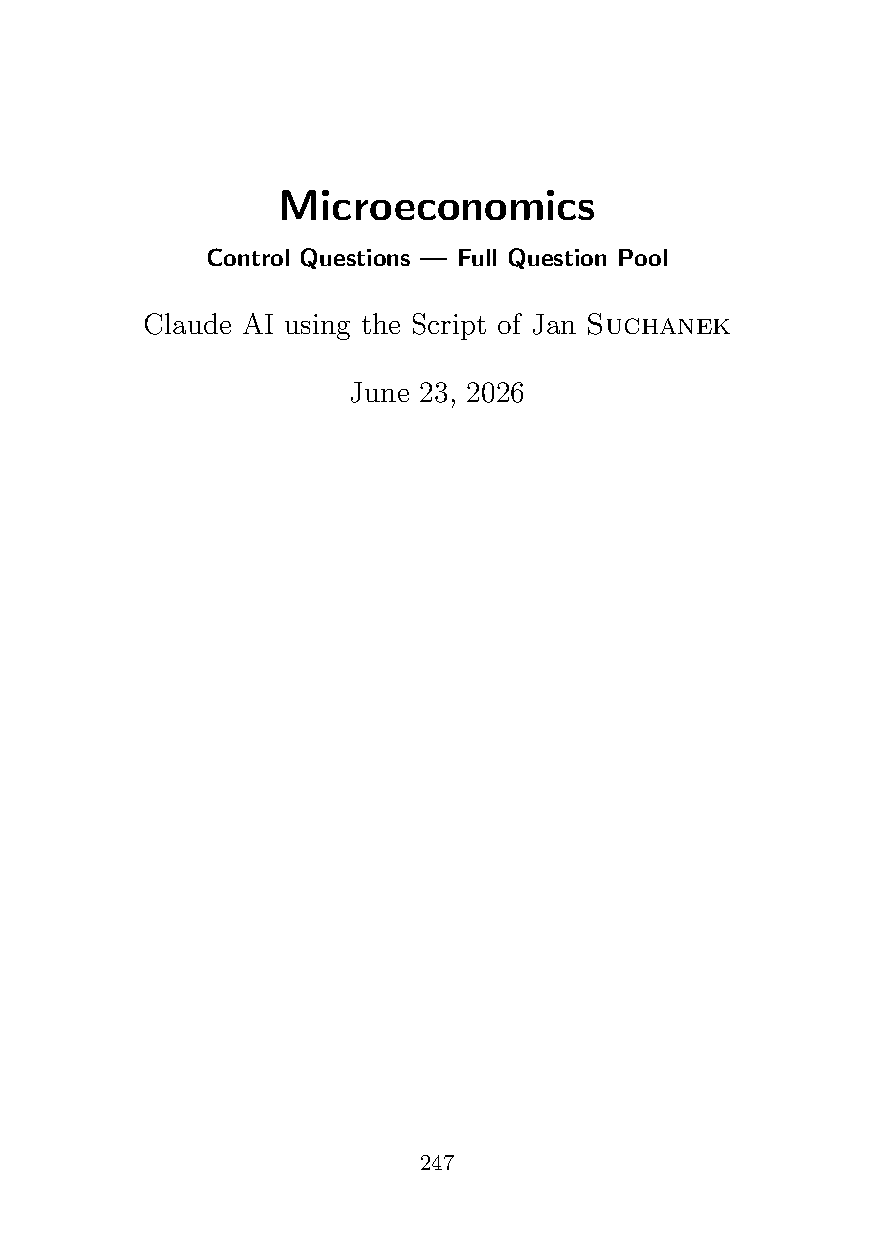
\includepdf[pages=-]{microeconomics/questionbank/ME_QuestionPool.pdf}

\end{document}
